\documentclass[12pt,a4paper]{report}
\usepackage{cmap} %The cmap package is intended to make the PDF files generated by pdflatex "searchable and copyable" in acrobat reader and other compliant PDF viewers.

\usepackage[T1,T2A]{fontenc} %russian and latin encodings
\usepackage[utf8x]{inputenc} % UTF-8
\usepackage[english,russian]{babel} %english and russian langs
\usepackage{cite} % The pack­age sup­ports com­pressed, sorted lists of nu­mer­i­cal ci­ta­tions, and also deals with var­i­ous punc­tu­a­tion and other is­sues of rep­re­sen­ta­tion, in­clud­ing com­pre­hen­sive man­age­ment of break points. The pack­age is com­pat­i­ble with both hy­per­ref and back­ref.

%\usepackage[nottoc,numbib]{tocbibind}% http://en.wikibooks.org/wiki/LaTeX/Bibliography_Management 

\usepackage{geometry} % Меняем поля страницы
\geometry{left=2cm}% левое поле
\geometry{right=1.5cm}% правое поле
\geometry{top=1cm}% верхнее поле
\geometry{bottom=2cm}% нижнее поле



\usepackage{indentfirst} %Make the 1st line of all sections etc., be indented by the usual paragraph indentation. This should work with all the standard document classes.


\usepackage[onehalfspacing]{setspace} %Pro­vides sup­port for set­ting the spac­ing be­tween lines in a doc­u­ment. Pack­age op­tions in­clude sin­glespac­ing, one­half­s­pac­ing, and dou­blespac­ing. Al­ter­na­tively the spac­ing can be changed as re­quired with the \sin­glespac­ing, \one­half­s­pac­ing, and \dou­blespac­ing com­mands. Other size spac­ings also avail­able.

\usepackage{graphicx} %разрешить включение графики
\graphicspath{{../pictures/}} %относительный путь к каталогу с рисунками,  это может быть мягкая ссылка

\usepackage{hyperref}
\hypersetup{pdftitle={Statistics Done Wrong (in Russian)},pdfauthor={Alex Reinhart},pdfsubject={The woefully complete guide},pdfcreator={Pasha P. Komar},colorlinks=true,urlcolor=cyan,citecolor=blue,linkcolor=blue}
%%%%%%%%%%%%%%%%% end of preamble%%%%%%%%%%%%%%%%%%%%%%%%%%%\\

%%%%%%%%%%% NEW PACKAGES%%%%%%%%%%%%%%%%%%%%%%%%

%\usepackage{makeidx} %making index
%\makeindex % команда для создания предметного указателя


%%%%%%%%%% command for an epigraph %%%%%%%%%%%%%%%%%%%
\makeatletter
\renewcommand{\@chapapp}{}% Not necessary...
\newenvironment{chapquote}[2][2em]
  {\setlength{\@tempdima}{#1}%
   \def\chapquote@author{#2}%
   \parshape 1 \@tempdima \dimexpr\textwidth-2\@tempdima\relax%
   \itshape}
  {\par\normalfont\hfill--\ \chapquote@author\hspace*{\@tempdima}\par\bigskip}
\makeatother
%%%%%%%%%%%%% end of epigraph %%%%%%%%%%%%%%%


%%%%%%%%%%%%%%%%%%%%%%%%%%%%%

\begin{document}

%\frontmatter

\title{Считаем статистику неправильно\\ \emph{Удручающе полное руководство}}
\author{Алекс Рейнарт\\ \url{http://statisticsdonewrong.com}}
\date{} 
\maketitle

\tableofcontents 


%% Основной текст %%
%\mainmatter
%%% Prologue %%%
\chapter*{Вступление}
\label{chp0}
\addcontentsline{toc}{chapter}{Вступление}
Если вы - учёный, возможно, в своей деятельности используете статистику для анализа данных. При поиске ответов на научные проблемы мы полагаемся на статистику, начиная с базовых t-тестов или подсчёта стандартной ошибки и заканчивая регрессией Кокса и методом подбора контрольной группы по индексу соответствия. %перевод термина - https://ru.wikipedia.org/wiki/%DD%EA%EE%ED%EE%EC%E5%F2%F0%E8%F7%E5%F1%EA%E8%E5_%EC%E5%F2%EE%E4%FB_%E2_%EE%F6%E5%ED%E8%E2%E0%ED%E8%E8#.D0.9C.D0.B5.D1.82.D0.BE.D0.B4_.D0.BF.D0.BE.D0.B4.D0.B1.D0.BE.D1.80.D0.B0_.D0.BA.D0.BE.D0.BD.D1.82.D1.80.D0.BE.D0.BB.D1.8C.D0.BD.D0.BE.D0.B9_.D0.B3.D1.80.D1.83.D0.BF.D0.BF.D1.8B_.D0.BF.D0.BE_.D0.B8.D0.BD.D0.B4.D0.B5.D0.BA.D1.81.D1.83_.D1.81.D0.BE.D0.BE.D1.82.D0.B2.D0.B5.D1.82.D1.81.D1.82.D0.B2.D0.B8.D1.8F

Это прискорбно, поскольку большинство из нас просто не умеет делать статистические подсчёты.

\emph{Неправильная статистика} - это руководство, описывающее популярные статистические ошибки и просчёты, которые совершают учёные ежедневно в лабораториях или в рецензируемых журналах. Многие из этих ошибок настолько распространены в научной литературе, что ставят под сомнение результаты большого количества статей.

Эта книга не предполагает наличие у читателя никаких статистических знаний: вы можете прочитать её перед своим первым курсом по статистике или после 30 лет научной деятельности.

Если вы обнаружите какие-либо ошибки, опечатки или можете предложить другие популярные заблуждения по теме -  \hyperref[chp1:contact]{свяжитесь со мной}. 

В попытке создать наиболее полную коллекцию статистических ошибок, я заключил контракт на публикацию \emph{Неправильной статистики} в виде расширенной книги, включающей новые разделы о статистическом моделировании, дополнительных математических разъяснениях и многом другом. \href{http://statisticsdonewrong.com}{Здесь} можно подписаться рассылку по электронной почте, а если сайт оказался вам полезным, может быть вам также понравится \href{http://www.nostarch.com/statsdonewrong}{моя книга} - она уже опубликована.


%% Chapter 1 %%%
\chapter{Введение}
%\addcontentsline{toc}{chapter}{Введение}
\label{chp1}

В заключительной главе своей знаменитой книги \emph{"Лгать с помощью статистики"} Дэррел Хафф говорит нам, что "любые статьи, имеющие отношение к медицине" или опубликованные научными лабораториями и университетами, заслуживают нашего доверия - не безусловного, но, определённо большего, чем публикации СМИ или заявления политиков. Всё же книга Хаффа была посвящена вводящим в заблуждение статистическим трюкам и ухищрениям, так часто используемыми в политике и СМИ, но мало кто выражает недовольство о качестве статистики, выполняемой профессиональными учеными. Ученые ищут ответы на вопросы, а не защиту от политических оппонентов.


Статистический анализ данных - это основа науки. Откройте любую страницу вашего любимого медицинского журнала и удивитесь популярности статистики: \emph{t} тесты, \emph{p}-значения, модели пропорциональных рисков, относительные риски, логистические регрессии, методы наименьших квадратов и доверительные интервалы. Статистики дали учёным функциональные инструменты для организации и анализа сложных наборов данных, и учёные их с удовольствием приняли.
 
Не приняли они, однако, сопутствующее статистическое \emph{образование}, и многие бакалаврские программы до сих пор не требуют вообще никакой статистической подготовки.

Начиная с 1980-х годов, исследователи описали множество статистических ошибок и заблуждений, встречающихся в популярной рецензируемой научной литературе, и обнаружили, что многие научные статьи - возможно, даже большинство, - стали жертвами этих ошибок. Недостаточная статистическая мощность отражает многие исследования, неспособные найти искомое; множественные сравнения и неверно интерпретированные \emph{p}-значения приводят к многочисленным ошибкам первого рода; гибкий анализ данных с лёкостью позволяет найти корреляцию там, где её не существует. Проблема не в подделывании результатов, а в низком уровне владения статистикой - настолько низком, что некоторые учёные делают вывод, что большинство опубликованных результатов исследований, скорее всего, ошибочны.\cite{ioannidis_why_2005}

Далее следует список наиболее вопиющих статистических ошибок, совершаемых регулярно во имя науки. Он не предполагает знания статистических методов, поскольку многие учёные вообще не получали формальной статистической подготовки. И имейте в виду: едва познакомившись с этими ошибками, вы будете встречать их \emph{везде}. Не пугайтесь. Это не повод отказываться от современной науки и обращаться заново к кровопусканию и лечению пиявками: это попытка улучшить науку, на которую мы полагаемся.
 

\section{Изменения}
\label{chp1:changes}

Обновлено в январе 2013: добавлен пример ошибки обоснования оценки: \hyperref[chp5:arms-baserateF]{подсчет количества владельцев оружия на основании опроса}.  

%%%%%%%%%%%%%%%%%%%%%%%%%%%%%%%%%%%%%%%%%%%%%%%
%%%%%%%%%%%%%%%%%%%%%%%%%%%%%%%%%%%%%%%%%%%%%%%%
%%%%%%%%%%%%%%%%%%%%%%%%%%%%%%%%%%%%%%%%%%%%%%%%
Обновлено в апреле 2013: более подробно рассказано о \hyperref[chp7:truthinflation]{взаимодействии преувеличения истины (truth inflation) и правилах предварительной остановки (early stopping rules)}, \hyperref[chp5:redherrings]{свободе исследователя в нейронауках}, \hyperref[chp3:powerunderpowered]{слабой статистической мощности в нейронауках}, \hyperref[chp5:controlfalserate]{контроле коэффициентов ложных обнаружений}, \hyperref[chp10]{искажениях в публикациях и слабых отчётах}, \hyperref[chp3:wrongturnred]{слабых исследованиях и правых поворотах на красный свет}, \hyperref[chp6:significantdiffmissed]{неправильном использовании доверительных интервалов},\hyperref[chp11]{
влиянии всех этих ошибок}, \hyperref[chp12]{о том, что можно сделать, чтобы спасти статистику}, и добавлены дополнительные ссылки и подробности в разных частях книги.

%%%%%%%%%%%%%%%%%%%%%%%%%%%%%%%%%%%%%
%%%%%%%%%%%%%%%%%%%%%%%%%%%%%%%%%%%%%
%%%%%%%%%%%%%%%%%%%%%%%%%%%%%%%%%%%%%

\section{Контакты}
\label{chp1:contact}

Я старался изо всех сил, но эта рукопись неизбежно содержит ошибки и упущения. Если у вас возникли вопросы, вы заметили ошибку или знаете что-то, что упустил я, - \href{mailto:alex@refsmmat.com}{напишите мне}\footnote{Если заметили неточности или ошибки в переводе - напишите \href{https://github.com/cellahchain/statisticsdonewrong}{переводчику.}}.

\section{Благодарности}
\label{chp1:acknow}

Спасибо д-ру Джеймсу Скотту (James Scott), чей курс по статистике дал мне основы, необходимые для написания этого текста; Мэттью Уотсону (Matthew Watson) и CharonY за неоценимую обратную связь и предложения в процессе написания этого текста; моим родителям - за отзывы и предложения; д-ру Бренту Айверсону (Brent Iverson), семинары которого побудили меня заинтересоваться злоупотреблением статистикой; и всем тем учёным и статистикам, которые, совершая ошибки, дали мне повод об этом написать.

Любые ошибки в объяснениях - мои собственные, или неточности перевода.

\section{Лицензирование}
\label{chp1:copyleft}

Эта работа предоставлена под лицензией Creative Commons Attribution 3.0 Unported \href{http://creativecommons.org/licenses/by/3.0/}{License}.

Вы можете свободно печатать, копировать, переводить, переписывать, накладывать на музыку и, в целом, делать всё что угодно с этой работой при условии, что вы ссылаетесь на меня, Alex Reinhart, и указываете ссылку на \href{http://statisticsdonewrong.com}{сайт}. (Если вы сделаете перевод, пожалуйста, сообщите мне! Я с удовольствием размещу ссылку на ваш перевод.) Подробнее о лицензии можно узнать по ссылке выше.

Используемые в тексте картинки xkcd доступны под лицензией Creative Commons Attribution NonCommercial 2.5 \href{http://creativecommons.org/licenses/by-nc/2.5/}{License} и не могут использоваться в коммерческих целях без разрешения их авторов. Подробнее \href{http://xkcd.com/license.html}{здесь}. %Введение и вступление
%% Section 2 %%% Введение в анализ данных


\chapter{Введение в анализ данных}
\label{chp2}

Большая часть экспериментальной науки сводится к измерению каких-либо изменений. Действует ли одно лекарство лучше другого? Синтезируют ли клетки с одним набором генов большее количество ферментов, чем клетки с другим набором? Какой из алгоритмов обработки сигнала лучше обнаруживает пульсары? Является ли один катализатор эффективнее другого?

Таким образом, большинство статистических расчётов сводится к принятию решения о том, существуют ли различия между измерениями. Мы говорим о т.н. "статистически значимых различиях"\hspace{1pt}, поскольку статистики изобрели методы, позволяющие определять ситуации, когда различия между несколькими измерениями значимы - т.е. невозможно утверждать, что эти различия возникли случайным образом.

Допустим, вы хотите протестировать эффективность средств от простуды. Некоторое новое лекарство, предположительно, сокращает продолжительность проявления симптомов простуды на 1 день. Чтобы проверить данное утверждение, вы находите 20 пациентов со схожими симптомами, делите их на равные группы; одной группе предлагаете новое лекарство, а другой - плацебо. Далее вы отслеживаете продолжительность проявления симптомов простуды у каждой группы и подсчитываете ее среднее значение для каждой из групп.

Но не все простуды одинаковы. Возможно, простуда у человека длится около недели, в среднем, но у некоторых она может продолжаться всего несколько дней, в то время как у других - 2 недели и более, серьезно истощая домашние запасы салфеток. Вполне вероятно, что та группа из 10 человек, которая получала лекарство, могла состоять как раз из таких счастливчиков с двухнедельной простудой, и тогда вы сделаете ошибочный вывод о том, что лекарство только ухудшает ситуацию.  Как определить, что мы доказали эффективность лекарства, а не то, что мы выбрали неудачную выборку для эксперимента?

\section{Мощность \emph{p}-значений}
\label{chp2:pvalues}

Статистика дает ответ на этот вопрос. Если нам известно \emph{распределение} случаев типичной простуды - примерное количество пациентов с симптомами краткосрочной простуды, длительной и средней по длительности простуды - мы можем оценить насколько вероятно то, что некая случайная выборка пациентов с простудой будет состоять из людей с продолжительностью простуды меньше, чем в среднем, больше, чем в среднем или идентично средней длительности. Используя статистический тест, мы можем ответить на вопрос: ``Если мое лекарство не подействовало, какова вероятность того, что я увижу такие же данные, что я уже видел?''
Звучит несколько сложно, поэтому, прочтите ещё раз.


Интуитивно, мы можем увидеть, как это должно работать. Если я проверю лекарство только на 1 человеке, вполне ожидаемо, если он вылечится быстрее, чем в среднем длится простуда, - просто потому, что у половины пациентов простуда длится меньше, чем в среднем у всех пациентов. Однако, если проверить лекарство на 10 миллионах пациентов, чертовски маловероятно, что \emph{все} они вылечатся быстрее, чем в среднем, \emph{если только моё лекарство не подействовало}.    

Общепринятые статистические тесты, используемые статистиками, выводят число, называемое \emph{p}-значением, которое это подсчитывает. Вот как оно определяется:

\begin{quotation}

\textbf{\emph{P}-значение}\footnote{Альтернативное определение из \href{http://goo.gl/JHujIw}{Википедии}: \textit{\textbf{p-значение} равно вероятности того, что случайная величина с данным распределением (распределением тестовой статистики при нулевой гипотезе) примет значение, не меньшее, чем фактическое значение тестовой статистики}.} можно определить как вероятность получить результат равный или больший, чем в реальности наблюдаемый, при условии, что никакого эффекта или различий обнаружено не было (нулевая гипотеза).\cite{goodman_toward_1999}   

\end{quotation}


Таким образом, если я дам свое лекарство 100 пациентам и увижу, что их простуды длятся на 1 день меньше, чем в среднем, р-значением такого результата будет вероятность того, что все мои 100 пациентов совершенно случайно имели простуду на 1 день короче, при условии, что моё лекарство не подействовало. Очевидно, что \emph{р}-значение зависит от размера эффекта (простуды, которые длятся на 4 дня меньше встречаются реже и менее вероятны, чем простуды, длящиеся на лишь 1 день меньше среднего значения) и от количества пациентов, на которых проверяется лекарство  


Это хитрое понятие, которое может запутать. \emph{P}-значение - не мера того, насколько вы правы или насколько значимы различия; скорее, оно измеряет то, \emph{насколько сильно вы должны быть удивлены} в случае, если никаких реальных различий между группами обнаружено не будет, а у вас есть данные, предполагающие обратное. Чем больше различия или чем больше данныих, подкрепляюших эти различия, тем больше степень удивления и меньше \emph{р}-значение.

Не так уж просто превратить это в ответ на вопрос: “а существуют ли в реальности различия?” Большинство ученых используют простое эмпирическое правило: если \emph{р}-значение меньше 0,05, существует только 5\% шанс получения такого результата, когда лекарство действительно не работает, - поэтому мы станем считать различия между лекарством и плацебо ``значимыми''. Если \emph{р}-значение больше, различия будут считаться незначимыми.

Но здесь существуют ограничения. \emph{Р}-значение - это мера нашей степени удивления, а не размер эффекта. Я могу получить крошечное р-значение либо измеряя огромный эффект - ``наше лекарство увеличивает продолжительность жизни людей в 4 раза'', либо измеряя очень маленький эффект с большой достоверностью. Статистическая значимость не означает, что ваш результат имеет какую-либо \emph{практическую} или \emph{фактическую} значимость.

Аналогичным образом сложно интерпретировать и статистическую \emph{не}значимость. У меня может быть прекрасное лекарство, но если я протестирую его всего на 10 пациентах, мне будет очень трудно определить, откуда взялись различия: вследствие реального действия лекарства или моей удачи. Или я мог бы попеременно протестировать лекарство на тысячах пациентов, а лекарство укорачивало бы простуду всего на 3 минуты, поэтому я просто был бы не в состоянии отследить такие различия. Статистически незначимое различие не означает, что в реальности различий не существует.

К сожалению, нет такого математического инструмента, который позволил бы определить, верна ли ваша гипотеза; вы можете только проверить, согласуется ли эта гипотеза с данными - и если данные беспорядочны или маловразумительны, ваши выводы будут такими же. 

Но нас это не остановит. %Введение в анализ данных
%% Section 3 %%%
%\chapter[toc version]{doc version} % эта строка позволяет задать разные названия главы для оглавления и самого документа;


\chapter[Статистическая мощность]{Статистическая мощность и недостаточно мощные статистики}
\chaptermark{Статистическая мощность}% а эта - предписывает название в header на страницах этой главы, http://tex.stackexchange.com/questions/6862/how-can-i-display-a-short-chapter-name-in-the-header-and-a-long-chapter-name-in
\label{chp3}

Мы уже ранее видели, как можно не заметить реальный эффект, взяв недостаточное количество данных. В большинстве случаев это и есть основная проблема: мы можем упустить потенциально действующее лекарство или не заметить серьезный побочный эффект. Как определить, какое количество данных необходимо собрать? 

Отвечая на этот вопрос, статистики используют понятие ``статистическая мощность''. Мощность исследования - это вероятность того, что оно сможет отличить прояление эффекта определенного размера от случайного удачного исхода. Исследование может легко определить огромную пользу какого-либо лекарства, но в меньшей степени способно заметить едва уловимые различия. Давайте рассмотрим простой пример.

Предположим, что игрок убежден в том, что у его оппонента неправильная монета: количество выпадающих орлов и решек у этой монеты отличается от нормального и оппонент этим пользуется, чтобы жульничать в невероятно скучных играх по подбрасыванию монетки. Как это доказать?

Нельзя просто подкинуть монетку 100 раз и подсчитать количество раз, когда выпал орёл. Даже подбрасывая идеальную монетку, вы не всегда получите ровно 50 выпавших орлов: 


\newpage % делаем разрыв, чтобы картинка была первой на след странице

%%%%%%%%%%%%%% figure 1 %%%%%%%%%%%%%%%%%%5
\begin{figure}[h!]
    \centering
    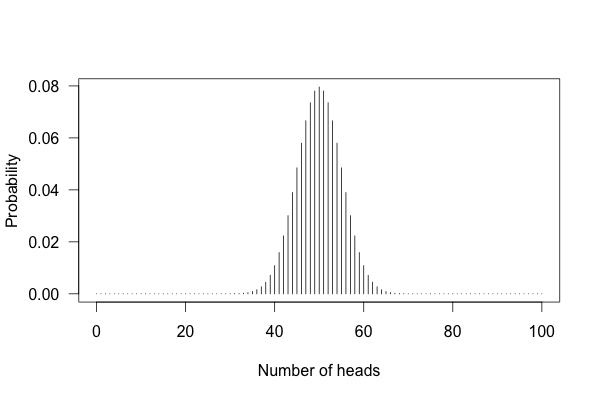
\includegraphics[width=0.8\textwidth]{binomial}
    \caption{На рисунке изображена вероятность (probability) выпадения различного количества орлов (number of heads), если подбросить монетку 100 раз.}
    \label{fig3:binominal}
\end{figure}
%%%%%%%%%%%%%%% end of figure 1 %%%%%%%%%%%%%%%%%%%

Из рисунка видно, что выпавшие 50 раз орлы - это наиболее вероятный исход 100 раз подбрасывания монетки, однако также вполне вероятно и выпадение орла 45 или 57 раз. Если орел выпал 57 раз, причиной тому может быть как неправильная монета, так и просто ваше везение.  

Давайте обратимся к математике. Возьмем, к примеру, \emph{р}-значение равное 0,05 или менее, как обычно делают ученые. То есть, если я посчитаю количество выпавших орлов после 10 или 100 подбрасываний монеты и обнаружу различия с ожидаемым результатом (орел и решка должны выпасть равное количество раз), тогда я смогу назвать монету неправильной, поскольку существует только 5\% шанс получить такое или большее различие, используя нормальную монету. В противном случае, я вообще не могу сделать никакого вывода: может быть монета нормальная, а может быть она немного неправильная, я не могу этого сказать.

Таким образом, что произойдет, если я подброшу монету 10 раз и применю эти рассуждения?


\newpage % делаем разрыв, чтобы картинка была первой на след странице

%%%%%%%%%%%%%% figure 2 %%%%%%%%%%%%%%%%%%5
\begin{figure}[h!]
    \centering
    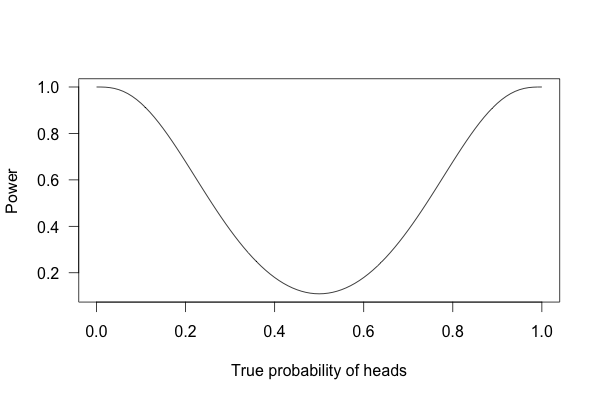
\includegraphics[width=0.8\textwidth]{power-curve-10}
    \caption{Истинная вероятность выпадения орлов}
    \label{fig3:powercurve10}
\end{figure}
%%%%%%%%%%%%%%% end of figure 2 %%%%%%%%%%%%%%%%%%%

Этот рисунок отображает т.н. \emph{функцию мощности}. На горизонтальной оси расположены различные значения, которые может принимать истинная вероятность выпадения орлов, соответствующие разным уровням несправедливости. На вертикальной оси - вероятность того, что я буду считать монету несправедливой (неправильной) после 10 подбрасываний, основываясь на \emph{р}-значении результата.

Можно увидеть, что если монета неправильная и ``подкручена'' на результат в 60\% постоянно выпадающих орлов, а я подбрасываю монету 10 раз, у меня есть лишь 20\% шанс сделать вывод о том, что монета неправильная. В данном случае, у меня слишком мало данных, чтобы отличить неправильную монету от случайности. Чтобы постоянно замечать это, монета должна быть слишком неправильной.

Но что будет, если я подброшу монету 100 раз?

\newpage % делаем разрыв, чтобы картинка была первой на след странице

%%%%%%%%%%%%%% figure 3 %%%%%%%%%%%%%%%%%%5
\begin{figure}[h!]
    \centering
    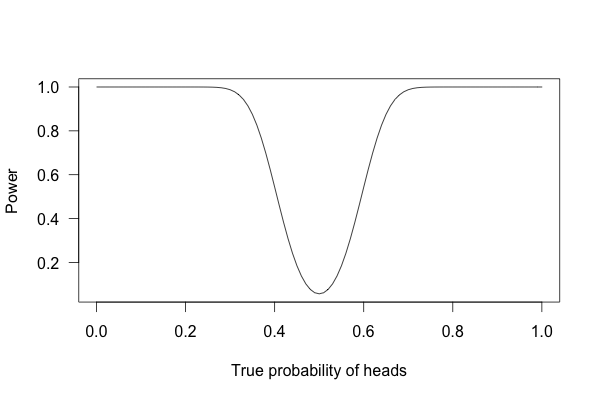
\includegraphics[width=0.8\textwidth]{power-curve-100}
    \caption{Истинная вероятность выпадения орлов}
    \label{fig3:powercurve100}
\end{figure}
%%%%%%%%%%%%%%% end of figure 3 %%%%%%%%%%%%%%%%%%%


А 1000 раз?
%\newpage % делаем разрыв, чтобы картинка была первой на след странице

%%%%%%%%%%%%%% figure 4 %%%%%%%%%%%%%%%%%%5
\begin{figure}[h!]
    \centering
    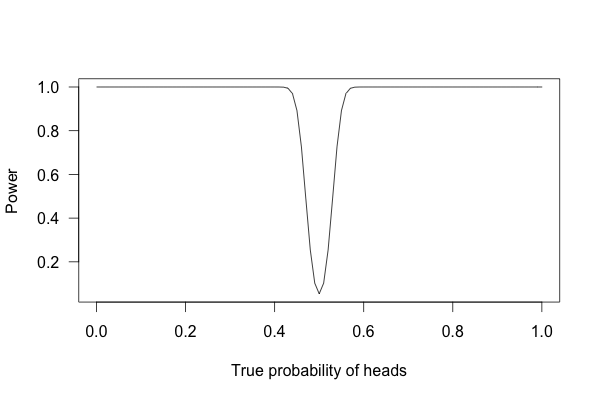
\includegraphics[width=0.8\textwidth]{power-curve-1000}
    \caption{Истинная вероятность выпадения орлов}
    \label{fig3:powercurve1000}
\end{figure}
%%%%%%%%%%%%%%% end of figure 4 %%%%%%%%%%%%%%%%%%%

Подбрасывая монету 1000 раз, я смогу легко понять, ``подкручена'' ли монета на 60\% постоянного выпадения орлов. Крайне маловероятно, что подбрасывая нормальную монету 1000 раз я смогу получить более 600 выпавших орлов.



%%%%%%%%%%%%% new section %%%%%%%%%%%%%%%%%%%%%%%
\section[Недостаточная мощность]{Недостаточная мощность}
\label{chp3:powerunderpowered}

Дочитав до этой строки, у вас может сложится впечатление, что подсчет статистической мощности должен быть неотъемлимой частью клинических испытаний. Учёный, возможно, захочет узнать, какое количество пациентов должно участвовать в испытаниях, при условии, что новое лекарство повышает выживание более чем на 10\%, и он бы получил ответ, быстро рассчитав статистическую мощность. Учёные, обычно, вполне удовлетворены статистической мощностью в 0,8 и более, что соответствует шансу в 80\% сделать вывод о том, что наблюдался реальный эффект. 

Тем не менее, едва ли кто-либо из ученых когда-либо совершал эти подсчеты, и лишь некоторые статьи изредка указывают статистическую мощность используемых тестов.

Давайте рассмотрим эксперимент, направленный на тестирование двух различных лекарств в одинаковых условиях. Вы, возможно, хотели бы узнать, какое из лекарств будет безопаснее, но, к сожалению, побочные эффекты очень редко встречаются. Вы можете протестировать каждое из лекарств на сотнях пациентов, но только у некоторых из них проявятся заметные побочные эффекты.

Естественно, у вас не будет достаточного количества данных, чтобы сравнить оба лекарства по данному критерию: если в одной группе только у 4 пациентов проявились серьезные побочные эффекты, а в другой - только у троих, едва ли вы сможете понять, является ли лекарство причиной их проявлений.


К сожалению, многие эксперименты делают вывод о том, что ``Статистически значимых различий между группами в проявлении побочных эффектов не обнаружено'', не отмечая тот факт, что у них было достаточных данных для обнаружения небольших различий.\cite{tsang_inadequate_2009} И поэтому врачи ошибочно считают, что оба лекарства одинаково безопасны, в то время как одно из них может иметь гораздо опаснее другого.

Можно подумать, что подобная проблема возникает только в ситуациях, когда лекарство имеет слабый эффект, но это не так. В подборке исследований, опубликованных между 1975 и 1990 гг. в престижных медицинских журналах, в 27\% рандомизированных контроллируемых испытаниях были получены отрицательные результаты, но 64\% из них не собрали достаточного количества данных для обнаружения пятидесятипроцентной разницы между тестируемыми группами по основному показателю!!! 50\%!!! Даже если одно из лекарств снижает симптомы на 50\% лучше, чем другое лекарство, данных все равно недостаточно, чтобы признать его более эффективным. И 84\% исследований, получивших отрицательные результаты, не обладали достаточной статистической мощностью, чтобы определить и различия в 25\%. \cite{moher_statistical_1994,bedard_statistical_2007,brown_1987,chung_1998}

В нейронауках, ситуация выглядит гораздо хуже. Предположим, мы соберем в единое данные из множества нейронаучных статей, изучающих один и тот же эффект и уверенно оценивающих размер этого эффекта. Если взять медианное исследование, у него будет только 20\% шанс обнаружить этот эффект. Только после аггрегации множества исследований, данный эффект можно было заметить. Схожие проблемы возникают и в нейронаучных исследованиях, использующих моделирование животных - что формирует значительную этическую проблему: если каждое исследование в отдельности не имеет достаточной статистической мощности, эффект может быть обнаружен только после проведения большого количества исследований (и использования большого количества животных), в то время как можно всего лишь должным образом провести первое исследование.\cite{button_power_2013}

Не говоря уже о том, что ученые лгут, когда заявляют, что они не обнаружили значимых различий между группами. Вы лишь обманываете себя, когда предполагаете, что это означает отсутствие \emph{реальных} различий. Различия могут существовать, но ваше исследование было слишком маленьким, чтобы их заметить.

Вот еще один пример, который мы наблюдаем ежедневно.

\section{Поворот на красный сигнал}
\label{chp3:wrongturnred}

В 1970-х во многих частях США стали разрешать водителям поворачивать направо на красный сигнал светофора. До этого момента, в течении долгого времени проектировщики дорог и инженеры спорили о том, приведёт ли это к увеличению ДТП, в том числе, с участием пешеходов. Но разразившийся в 1973 году нефтяной кризис и его последствия побудили политиков рассматривать вопрос о разрешении поворота на красный сигнал исходя из идеи экономии горючего, которое впустую использовалось, в ожидании разрешающего сигнала светофора. 

Для изучения этого вопроса было проведено несколько исследований. Например, консультант департамента автомагистралей и транспорта Вирджинии провел т.н. ``до и после'' исследование двадцати перекрёстков, на которых разрешили поворот направо на красный сигнал светофора. За примерно одинаковый промежуток времени до разрешения на этих перекрестках произошло 308 ДТП, а после разрешения - 337. Однако, это различие не было статистически значимым, и поэтому консультант сделал вывод, что никакого влияния на безопасность дорожной ситуации разрешение поворота на красный сигнал не имело.

Несколько последующих исследований получили схожие результаты: небольшое увеличение в количестве ДТП, но этих данных было недостаточно для того, чтобы сделать вывод о значимом ухудшении ситуации. Один из отчетов подвел итог таким образом: 

\begin{quotation}
Нет ни единой причины считать, что количество ДТП с участием пешеходов и машин, поворачивающих на красный сигнал светофора направо, увеличилось с момента разрешения поворота направо на красный сигнал\dots
\end{quotation}

Основываясь на этих данных, все больше городов и штатов стали разрешать поворот направо на красный сигнал светофора. Проблема, естественно, заключается в том, что все проводившиеся исследования обладали низкой мощностью. Все большее количество пешеходов были сбиты автомобилями и все большее количество автомобилей участвовало в ДТП, однако никто не мог собрать достаточное количество данных, чтобы убедительно это доказать, до тех пор, пока исследования не стали давать отчетливые результаты: спустя несколько лет стало очевидно значительное увеличение ДТП (в некоторых случаях до 100\%) с участием машин и пешеходов.\cite{hauer_harm_2004,preusser_effect_1982} Такое ошибочное толкование исследований с недостаточной мощностью стоило человеческих жизней.  
 %
%% Chapter 4 %%%
\chapter{Псевдорепликация: выбирайте данные корректно}
\label{chp4}

Многие исследования стараются собрать больше данных путем репликации: повторяя свои измерения на дополнительных пациентах или выборках, они стремятся к подтвердить свои результаты и увидеть едва заметные взаимосвязи, которые не так очевидны на первый взгляд. Мы уже видели, насколько ценными могут быть дополнительные данные для улучшения статистической мощности и обнаружения небольших различий. Но что именно можно считать репликацией?

Воспользуемся снова медицинским примером. У меня есть 2 группы пациентов общим количеством в 100 человек, принимающие разные лекарства, и я пытаюсь установить, какое из лекарств лучше понижает кровяное давление. Чтобы увидеть результат, каждая из групп принимала лекарства в течении месяца, а потом я наблюдал за каждой из групп в течении 10 дней, ежедневно измеряя их давление. Таким образом, у меня есть по 10 переменных на каждого пациента и 1000 переменных на каждуюу группу. 

Замечательно! 1000 переменных - это достаточно много данных, и я могу относительно просто установить, уменьшилось ли давление у одной группы, по сравнению с другой. Если посчитать статистическую значимость различий - они определенно будут значимыми.

Однако, мы считали, что измеряя 10 раз давление у пациента, мы должны получить десять примерно одинаковых результатов. Если один из пациентов генетически предрасположен на низкое давление, я 10 раз посчитал его предрасположенность. Если бы я собрал данные от 1000 независимых пациентов вместо последовательного измерения 100 пациентов, я мог быть более уверен в том, что различия между группами являются следствием действия лекарства, а не генетики и случайной удачи. Я заявляю о большом размере моей выборки, которая дает мне статистически значимые результаты и высокую статистическую мощность, но это заявление неоправданно.  

Эта проблема часто встречается и известна под названием псевдорепликация.\cite{lazic_problem_2010} Протестировав несколько клеток одного микроорганизма, биолог может ``реплицировать'' свои результаты путем тестирования большего количества клеток из того же микроорганизма. Нейроучёные могут исследовать большое количество нейронов одного и того же животного, заявляя ошибочно, что у них была огромная выборка, потому что они исследовали несколько сотен нейронов из всего двух крыс.

В терминах статистики, псеворепликация происходит тогда, когда индивидуальные наблюдения сильно зависят друг от друга. Например, ваши измерения кровяного давления пациента будут тесно связаны с предыдущими измерениями, а результаты изучения состава почвы в одном месте будут положительно коррелировать с составом почвы в полуторах метрах от этого места. Существует несколько способов учета этой зависимости в процессе статистического анализа:

\begin{enumerate}
	\item Усреднение зависимых переменных. Например, можно усреднить все измерения кровяного давления у одного пациента, хотя это и не идеальный способ: если вы измеряли одних пациентов чаще, чем других, - это не отразится на среднем значении. Вам нужен будет метод, который каким-то образом будет учитывать следующее: чем больше измерений - тем более они надежны.
	\item Анализ каждой зависимой переменной по-отдельности. Можно использовать для анализа показания кровяного давления каждого пациента на пятый день, что даст только одну переменную на каждого пациента. Но здесь нужно быть осторожным, потому что если сделать это для каждого дня тестирования, могут возникнуть проблемы с \hyperref[chp5:try-again]{множественными сравнениями}, которые мы будем обсуждать в следущей главе.
	\item Использование статистических моделей, которые учитывают зависимые переменные, например, иерархическая модель данных или модель случайных эффектов.
\end{enumerate}  


Важно рассмотреть каждый из возможных подходов прежде, чем анализировать свои данные, поскольку каждый из методов лучше подходит к разным ситуациям. Псевдорепликация позволяет достичь статистической значимости довольно просто, хотя и не даёт никакой дополнительной информации об испытуемых. Исследователи должны быть аккуратны в своих выводах, не увеличивая искусственно размеры своей выборки путем повторного тестирования одной и той же выборки.
%% Chapter 5 %%%
\chapter[Ошибка базовой оценки]{\emph{Р}-значение и ошибка базовой оценки}
\label{chp5}
\chaptermark{Ошибка базовой оценки}

Как вы уже видели, \emph{р}-значения интерпретировать непросто. То, что мы получили статистически незначимые результаты, не означает, что различий не существует. А что означает статистически значимый результат?

Давайте посмотрим на примере. Предположим, я решил протестировать сотню потенциальных лекарств от рака. Только десять из них реально действуют, но я не знаю, какие именно - мне нужно проводить эксперименты, чтобы определить это. В самих экспериментах, я буду ориентироваться на $p<0,05$ в оценке различий с действием плацебо, что будет демонстрировать полезность тестируемого лекарства. 

Для иллюстрации, на изображении ниже каждая клетка таблицы представляет собой одно лекарство. Синим отмечены те клетки, которые соответствуют действующим лекарствам:


%\newpage % делаем разрыв, чтобы картинка была первой на след странице

%%%%%%%%%%%%%% figure 5 %%%%%%%%%%%%%%%%%%5
\begin{figure}[h!]
    \centering
    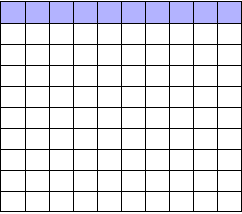
\includegraphics[width=0.4\textwidth]{drug-grids-1}
    %\caption{}
    \label{fig5:drug-grid-1}
\end{figure}
%%%%%%%%%%%%%%% end of figure 5 %%%%%%%%%%%%%%%%%%%

Как мы видили ранее, в большинстве испытаний сложно определить каждое хорошее лекарство. Давайте предположим, что статистическая мощность моих тестов - 0,8. Из десяти действующих лекарств, я смогу правильно распознать примерно 8 (отмечены фиолетовым на иллюстрации ниже):

\newpage % делаем разрыв, чтобы картинка была первой на след странице

%%%%%%%%%%%%%% figure 6 %%%%%%%%%%%%%%%%%%5
\begin{figure}[h!]
    \centering
    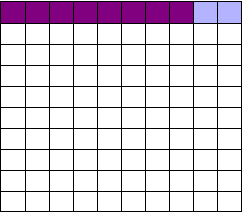
\includegraphics[width=0.4\textwidth]{drug-grids-2}
    %\caption{}
    \label{fig5:drug-grid-2}
\end{figure}
%%%%%%%%%%%%%%% end of figure %%%%%%%%%%%%%%%%%%%


Я также предположу, что около 5 из 90 недействующих лекарств будут иметь значимые эффекты. Почему? Напомню, что \emph{p}-значение подсчитывается исходя из предположения об отсутствии эффекта, т.е. $ p =0,05$ означает, что существует 5\% шанс сделать ошибочный вывод о том, что недействующее лекарство на самом деле действует.

Таким образом, я провожу свои эксперименты и делаю вывод о том, что у меня есть 13 действующих лекарств: 8 хороших лекарств и 5 тех, что я мог ошибочно включить в свой список (показаны красным на илюстрации ниже):


%\newpage % делаем разрыв, чтобы картинка была первой на след странице

%%%%%%%%%%%%%% figure 6 %%%%%%%%%%%%%%%%%%5
\begin{figure}[h!]
    \centering
    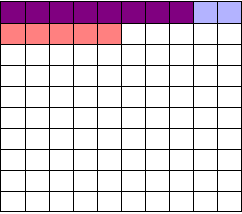
\includegraphics[width=0.4\textwidth]{drug-grids-3}
    %\caption{}
    \label{fig5:drug-grid-3}
\end{figure}
%%%%%%%%%%%%%%% end of figure %%%%%%%%%%%%%%%%%%%

Шанс того, что любое из ``действующих'' лекарств будет действительно эффективным, составляет только 6\%. Если бы я случайным образом выбрал одно лекарство из ста, провёл на нем свои тесты и обнаружил бы статистически значимую связь на уровне $p<0,05$, то существует всего 62\% шанса на то, что это лекарство действительно эффективно. Говоря терминами статистики, мои шансы совершить ошибку первого рода (оценка ложной тревоги) - это доля ложных положительных результатов в общем количестве статистически значимых результатов - составляют 38\%.  

Поскольку базовая оценка эффективности лекарств от рака довольно низкая - только около 10\% от множественных испытаний и лекарств дают какой-то результат, - большинство из тестируемых лекарств не действуют, и мы становимся особенно уязвимы к совершению ошибки первого рода. Будь я полным неудачником и будь у меня хоть целый грузовик совершенно бесполезных лекарств, базовая оценка эффективности которых составляет 0\%, я бы имел 0\% шанса на получение хоть какого-либо статистически значимого результата. Тем не менее, я все равно получу результат в $p<0,05$ для 5\% этих лекарств.

Часто можно слышать, как люди приводят в пример \emph{p}-значения в качестве показателя малой вероятности получения ошибки. ``Существует только 1 шанс из 10000, что такой результат возник случайным образом'' - говорят они, потому что получили значение $p=0,0001$. Увы, нет! Такое утверждение игнорирует базовую оценку, и встречается под названием \emph{ошибка базовой оценки}. Напомним, как определяется \emph{p}-значение:

\begin{quotation}

\textbf{\emph{P}-значение} можно определить как вероятность получить результат равный или больший, чем в реальности наблюдаемый, при условии, что никакого эффекта или различий обнаружено не было (нулевая гипотеза).   

\end{quotation}


\emph{P}-значение рассчитывается, основываясь на предположении о том, что лекарство \emph{не действует}, и даёт нам вероятность получения данных равных или больше тех, что мы получили. Оно не даёт нам вероятность того, что лекарство действует.

Когда кто-либо использует полученные \emph{p}-значения в качестве доказательства того, что они правы, запомните это. Вероятность ошибки их исследования, скорее всего, довольно высока. В сферах, где большинство проверяемых гипотез опровергаются, как, например, в первичных тестах лекарств (большинство таких лекарств не проходят тесты), вполне вероятно, что большинство ``статистически значимых'' результатов с $p < 0,05$ на самом деле всего лишь случайность.

Отличный пример тому - тесты на медицинскую диагностику.


\section[В медицинских испытаниях]{Ошибка базовой оценки в медицинских испытаниях}
\label{chp5:base-rateF}
\sectionmark{Медицинские испытания}

Существуют некоторые разногласия во мнениях по поводу использования маммографии при тестировании на рак груди. Некоторые считают, что опасность получить ложноположительный результат (и последующие ненужные биопсия, хирургическое вмешательство и химиотерапия) превышает те преимущества, которые даёт раннее обнаружение рака. Это статистический вопрос, давайте попробуем дать оценку.

Предположим, что у 0,8\% женщин, которым предписали маммографию, действительно  рак груди. У 90\% женщин, имеющих рак груди, маммография сможет его обнаружить. (Это статистическая мощность теста, но приблизительная, поскольку очень сложно сказать, сколько случаев рака груди мы упустили, если мы не знаем, что они вообще есть.) Тем не менее, из женщин, не имеющих рака груди, около 7\% получат ложноположительный результат на маммографии, ведущий к дальнейшим тестам, лечению и биопсии. Если вы получили положительный результат маммографии, каковы шансы на то, что у вас действительно рак груди?

Опуская те ситуации, когда ты, читатель, мужчина\footnote{Забавно, но если вы - мужчина, это не исключает возможности получить рак груди; это лишь делает вероятность чрезвычайно малой.}, ответ - 9\%.\cite{kramer_how_2005}

Несмотря на то, что тест даёт ложноположительный результат лишь у 7\% женщин, не имеющих рак груди, что аналогично $p < 0,07$, порядка 91\% положительных результатов на самом деле ложноположительные.

Как я это рассчитал? Точно таким же методом, как и в примере про лекарство от рака. Представьте себе 1000 случайно выбранных женщин, которые решили пройти маммографию. У восьми из них (0,8\%) есть рак груди. Маммография обнаруживает правильно около 90\% случаев рака, т.е. примерно у семи из восьми женщинрак будет обнаружен. Однако, остается 992 женщины без рака груди, и 7\% из них получат ложноположительный результат, т.е. у 70 женщин будет неверно диагностирован рак груди.

В сумме у нас получается 77 женщин с положительным результатом маммографии, у 7 из которых действительно есть рак груди. Только у 9\% женщин с положительным результатом по маммографии действительно есть рак груди.

Если задать этот вопрос студентам, изучающим статистику, и преподавателям научной методологи, более трети из них не смогут ответить верно.\cite{kramer_how_2005} Если задать его врачам, две трети из них провалятся на этом вопросе.\cite{bramwell_health_2006} Они ошибочно делают вывод о том, что $p < 0,05$ означает 95\% вероятность того, что результат истинный, хотя, как вы можете видеть из приведённых примеров, вероятность того, что положительный результат истиннен, зависит от того, какая часть проверенных гипотез верна. И нам просто повезло, что в любой момент времени рак груди возникает лишь у небольшой части женщин. 

Пролистайте вводные учебники по статистике и вы встретите подобное заблуждение довольно часто. \emph{P}-значения трудны для понимания, а ошибка базовой оценки встречается повсеместно.  


\section{Оружие против ошибки базовой оценки}
\label{chp5:arms-baserateF}
\sectionmark{Оружие против ошибки базовой оценки}

Чтобы столкнуться с этой ошибкой, нет нужды проводить расширенное исследование или тестировани на рак. А что, если вы делаете социологическое исследование? Например, вы хотите опросить американцев, чтобы узнать как часто они используют оружие в целях самообороны. В конце концов, в основе аргументов сторонников контроля оружия находится именно право на самозащиту, поэтому важно определить, используется ли оружие в большинстве случаев для защиты и перевешивает ли это недостатки, например, убийства.

Один из способов собрать необходимые данные - опрос. Можно опросить репрезентативную выборку американцев, узнав, владеют ли они оружием, и если да, использовали ли когда-нибудь оружие для защиты своего дома от незаконного проникновения или для защиты себя от ограбления. Затем можно сравнить полученные данные со статистикой правоохранительных органов об использовании оружия в случаях убийства и сделать вывод на основании этого вывод.

Такие опросы уже проводились, и результаты их довольно интересные. Один телефонный опрос, проведенный в 1992 году, позволил оценить, что американские граждане используют оружие в целях самообороны до 2,5 миллиона раз ежегодно - то есть, около 1\% американских взрослых защищали себя с помощью оружия. В 34\% случаях это была защита от незаконного проникновения в жилище, т.е. порядка 845000 взломов было остановлено владельцами оружия. Но за 1992 год было совершено только 1,3 миллиона взломов в дома, в которых кто-либо был. Две трети из них произошли в тот момент, когда жильцы дома спали, и сам факт взлома и ограбления был обнаружен уже после того, как воры покинули жилище. Получается, что остается порядка 430000 случаев взлома, когда домовладельцы были в доме и противостояли грабителям и, как нас пытаются убедить, в 845000 случаях из них, грабители были остановлены жителями - владельцами оружия.\cite{hemenway_survey_1996}   


Ой!


Что произошло? Почему опрос переоценил количество случаев использования оружия в целях самозащиты? По тем же причинам, что и маммография давала завышенную оценку случаев рака груди: гораздо больше возможностей для ложноположительных результатов, чем ложноотрицательных. Если 99,9\% людей никогда не использовали оружие в целях самообороны, но 1\% из них ответит ``да'' на любой вопрос просто ради забавы, еще 1\% ответит так, чтобы выглядеть более мужественно, а 1\% просто неправильно поймёт вопрос, - вы получите значительную переоценку использования оружия в целях самозащиты.

А что насчет ложноотрицательных результатов? Могут ли они быть сбалансированы людьми, которые говорили ``нет'', даже если они лично застрелили грабителя на прошлой неделе? Ответ: нет. Если лишь немногие действительно используют оружие в качестве самообороны, тогда возможность получить ложноотрицательные результаты слишком низка. Они вытесняются ложноположительными результатами.

Эта ситуация аналогична примеру с лекарствами от рака, описанному ранее. Здесь \emph{p}-значение - это вероятность того, что кто-нибудь будет ошибочно утверждать, что он использовал оружие в целях самообороны. Даже если значение \emph{p} будет небольшим, ваш окончательный ответ будет все равно неверным. 


Чтобы снизить \emph{p}-значение, криминологи используют более детальные опросы. Например, в исследованиях показателя национальной виктимизации населения (NCVS) используются подробные сидячие интервью с исследователями, где респондентов спрашивают о деталях преступлений и использования ими оружия в целях самообороны. Чем больше подробностей в опросе, тем лучше исследователи могут оценить, подходит ли конкретный инцидент под критерии самообороны. Результаты таких исследований гораздо скромнее - около 65000 случаев в год. Существует вероятность того, что эта оценка занижена, но и меньший шанс массовой переоценки.     


\section[Не удалось в первый раз - пробуйте еще]{Не удалось в первый раз - пробуйте еще}
\label{chp5:try-again}

Ошибка базовой оценки показывает, что ложноположительные результаты более вероятны в том случае, если вы считаете $p < 0,05$ критерием значимости. Большинство современных исследований не полагается только на один показатель значимости - они сравнивают эффекты нескольких факторов, надеясь найти один с наиболее значимыми эффектами.

Например, представьте себе исследование, в котором проверялось бы, являются ли драже причиной появления угревой сыпи на коже, путём исследования эффекта драже различного цвета: %см. \hyperref[fig5:xkcd-significant]{комикс xkcd}.

\newpage % делаем разрыв, чтобы картинка была первой на след странице

%%%%%%%%%%%%%% figure 7 %%%%%%%%%%%%%%%%%%5
\begin{figure}[h!]
    \centering
    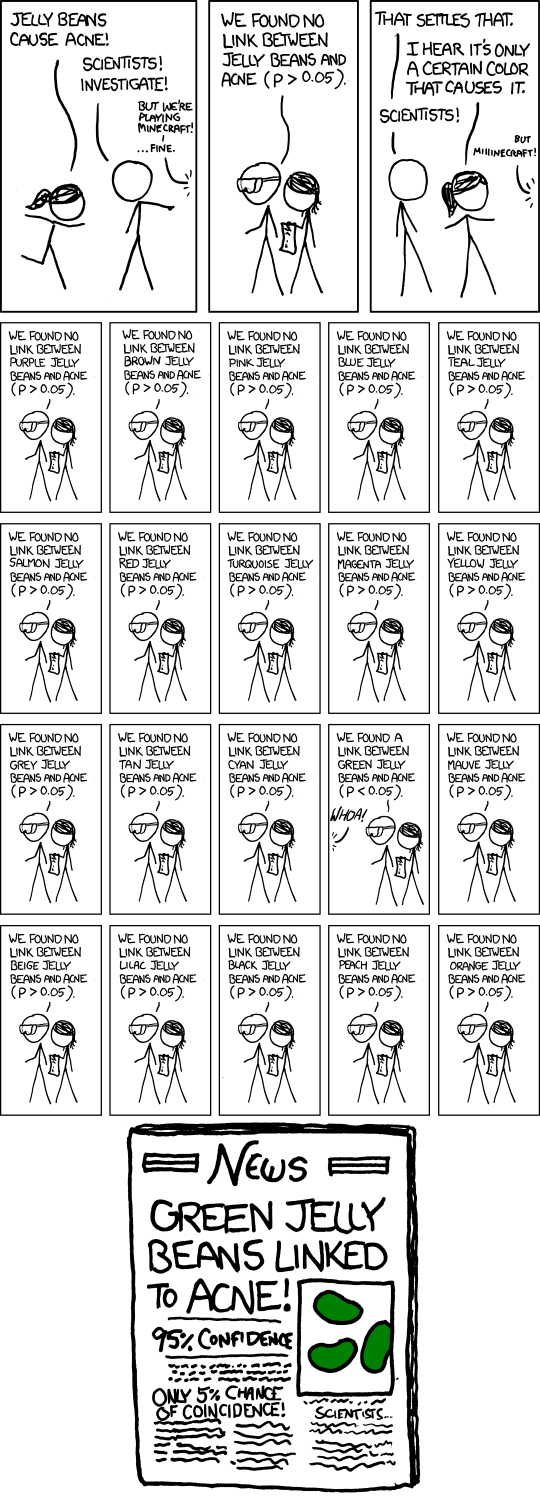
\includegraphics[width=0.5\textwidth]{xkcd-significant}
    \caption{xkcd-комикс, автор Randall Munroe. \href{http://xkcd.com/882/}{http://xkcd.com/882/}}
    \label{fig5:xkcd-significant}
\end{figure}
%%%%%%%%%%%%%%% end of figure %%%%%%%%%%%%%%%%%%%

Как видите, множественные сравнения подразумевают большое количество шансов получить ложноположительный результат. Например, если я буду исследовать 20 разных по вкусу драже, которые никаким образом не являются причиной появления угревой сыпи, и буду искать корреляцию с уровнем значимости $p < 0,05$, у меня будет 64\% шанс получить ложноположительный результат.\cite{smith_impact_1987} Если я проверю 45 различных драже, этот шанс вырастет до 90\%.

Множественные сравнения делать легко, и необязательно для этого, например, тестировать 20 потенциальных лекарств. Попробуйте отследить симптомы дюжины пациентов в течении дюжины недель и проверьте значимые различия в любой момент времени и вы получите 12 сравнений. Попробуйте проверить появление 23 потенциально опасных побочных эффекта и всё - вы уже согрешили. Разошлите десятистраничный опросник, выясняющий отношение людей к строительству атомной электростанции, потребление молока, возраст, количество кузенов, любимую пиццу, цвет носков и множество других хорошо измеряемых факторов, и вы найдете что-нибудь, что вызывает рак. Просто задайте достаточное количество вопросов, и обязательно что-нибудь найдётся.

Опрос на тему медицинских испытаний, проведённый в 1980-х, выявил, что за одно испытание, в среднем, делается около 30 терапевтических сравнений. В более чем половине испытаний исследователи делали настолько много сравнений, что вероятность получить ложноположительный результат была очень высока, а статистическая значимость результатов, о которых они сообщали, подвергалась сомнению: они, возможно, получали статистически значимые эффекты, но это могли быть и ложноположительные результаты.\cite{smith_impact_1987}

Существуют техники, позволяющие корректировать результаты в случае множественных сравнений. Например, метод коррекции Бонферрони утверждает, что если вы делаете $n$ сравнений в испытании, ваш критерий значимости должен быть $p < 0,05/n$. Это понижает шанс получить ложноположительный результат, по сравнению с ситуацией, когда вы делаете только одно сравнение на уровне $p < 0,05$. Однако, как можно себе представить, это снижает статистическую мощность, поскольку вам понадобятся более высокие кореляции для вывода о том, что они статистически значимы. Это сложный компромисс, и катастрофически малое количество статей его когда-либо вообще принимали во внимание.


\section{Ложный след в сканировании мозга} % английская идиома http://en.wikipedia.org/wiki/Red_herring 
\label{chp5:redherrings}

Нейроученые обычно делают огромное количество сравнений. Они часто проводят исследования с использованием фМРТ\footnote{Функциональная магнитно-резонансная томография}, где сравниваются трёхмерные изображения мозга, сделанные до и после того, как испытуемые выполняли какое-либо задание. Эти изображения показывают кровоток в мозгу, что позволяет выявить, какие участки мозга были наиболее активны в момент выполнения задания.

Но как определить, какие именно участки мозга были активны во время выполнения задания? Есть простой способ - разделить изображение мозга на небольшие кубические элементы, называемые вокселами. Воксел из изображения ``до'' сравнивается с вокселом из изображения ``после'', и если различия в кровотоке значительны, можно сделать вывод о том, что эта часть мозга была активна в момент выполнения задания. Проблема, однако, заключается в том, что сравниваемых вокселов - тысячи, а значит существует большой шанс получить ложноположительный результат.

В одном исследовании, к примеру, изучались эффекты ``умственного задания, допускающего неограниченное количество решений''. Участникам эксперимента показывали ``серию фотографий, на которых были изображены человеческие особи в социальных ситуациях с определенной эмоциональной валентностью,'' и просили их ``определить, какую эмоцию испытывает изображенный на фотографии субъект.'' Можете себе представить, насколько разные эмоциональные и логические центры мозга могли быть активными в процессе решения этого задания.   

Данные были проанализированы, и были замечены определенные участки мозга, изменяющие свою активность в процессе выполнения задачи. Сравнение изображений ``до'' и ``после'' дало различие на уровне значимости $p = 0, 001$ в 81 мм\textsuperscript{3} кластере мозга.

А участники исследования? Нет, это не были, как обычно, студенты вузов, участвующие в исследовании за 10\$. В качестве испытуемого выступал один 1,8 килограммовый атлантический лосось, который ``на момент сканирования не был жив''.\cite{bennett_neural_2009}  

Естественно, большинство нейронаучных исследований гораздо сложнее этого: существуют методы поиска кластеров вокселов, которые изменяются все вместе и одновременно, а также техники контроля возможных ложноположительных результатов даже в случае, когда проводятся тысячи статистических тестов. На данный момент, эти методы широко распространены в нейронаучной литературе, и те простые ошибки, что я описал, уже не так часто встречаются. Но, к сожалению, практически каждая статья решает проблему по-разному: обзор 241 исследования с использованием фМРТ показал, что в них были использованы 223 уникальные стратегии анализа, что, как мы обсудим позднее, \hyperref[chp8]{даёт огромную гибкость исследователям} получать статистически значимые результаты.\cite{carp_secret_2012}  


\section{Контроль оценки ложноположительных результатов}
\label{chp5:controlfalserate}

Ранее я упоминал, что существуют техники коррекции для множественных сравнений. Метод Бонферрони, например, предполагает, что можно правильно оценить ложноположительные результаты используя $p < 0,05/ n$, где $n$ - это количество статистических тестов, которые необходимо провести. Если проводить исследование, в котором делается двадцать сравнений, вы можете использовать пороговое значение в $p < 0,0025$ для уверенности в том, что есть только 5\% шанс ошибочно признать несуществующий эффект статистически значимым.

Однако, у этого метода есть недостаток. Понижая \emph{p}-значение , необходимое для признания результата статистически значимым, вы значительно понижаете статистическую мощность исследования, и легко можете упустить как реальный эффект, так и ложный. Существуют более сложные, чем коррекция Бонферрони, процедуры, которые используют преимущества определенных статистических свойств проблемы для увеличения статистической мощности, хотя и они не могут совершить магию. 

Хуже то, что они не избавляют вас от ошибки базовой оценки. Полученое \emph{p}-значение все еще может вводить вас в заблуждение, и вы ошибочно будете утверждать, что ``существует лишь 5\% шанс, что я ошибаюсь'', хотя вы лишь ликвидировали некоторые ложноположительные результаты. Ученые в большей степени заинтересованы в оценке ложноположительных результатов: какая часть моих статистически значимых результатов является ложноположительными? Существует ли какой-нибудь статистический тест, позволяющий мне контролировать эту часть? 

В течение длительного времени, ответ на этот вопрос был прост - ``нет''. Как вы видели в разделе об ошибке базовой оценки мы можем примерно оценить количество ложноположительных результатов, если мы предположим, какое количесто проверенных нами гипотез истинны, - однако, мы скорее узнаем это из полученных данных, чем будем угадывать. 

В 1995 году Бенджамини и Хохберг предложили более полезный ответ. Они разработали исключительно простую процедуру, которая может подсказать, какое \emph{p}-значение можно считать статистически значимым. До этого момента я старался избегать математических подробностей, однако цитата ниже иллюстрирует насколько проста эта процедура:

\begin{quotation}
Проведите необходимые статистические тесты и получите для каждого из них \emph{p}-значение. Составьте из них список в порядке возрастания.

Выберите оценку ложно положительных результатов и обозначьте её $q$, а количество статистических тестов $m$.

Найдите такое наибольшее \emph{p}-значение, соответствующее $p <= i*q/m$, где $i$ это порядковый номер \emph{p}-значения в упорядоченном выше списке.

Все \emph{p}-значения меньше или равные этому можно считать статистически значимыми. 
\end{quotation}  

Вот и всё! Процедура гарантирует, что из всех статистически значимых результатов, ложноположительных будет не более $q$ процентов.\cite{benjamini_controlling_1995}


Метод Бенджамини-Хохберга быстр и эффективен, и в определенных сферах стал широко применяться учеными и статистиками. Его использование даёт лучшую статистическую мощность, чем коррекция Бонферрони, кроме того, предоставляя более наглядные результаты. Он может использоваться в различных ситуациях, и варианты этой процедуры дают лучшую статистическую мощность на различных типах данных.

Конечно, метод не идеален. В некоторых странных ситуациях, он даёт довольно глупые результаты, и, как было математически доказано, всегда есть шанс того, что он может оказаться малополезным для контроля оценки ложноположительных результатов. Но это лучше, чем ничего, особенно для начала.

%% Chapter 6 %%%
\chapter{Различия в значимости $\neq$ значимые различия}
\label{chp6}

``Мы сравнили лекарство А и Б с действием плацебо. Лекарство А показало значительные улучшения, по сравнению с плацебо, в то время как лекарство Б не имело никаких статистически значимых преимуществ. Следовательно, лекарство А лучше лекарства Б''.

Мы слышим это постоянно. Таким образом легко сравнивать медикаменты, хирургические вмешательства, терапии и экспериментальные результаты. Это просто. И кажется, что это имеет смысл.

Тем не менее, разница в значимости не всегда даёт значимую разницу.\cite{gelman_difference_2006}

Представьте себе исследование, сравнивающее питание моржей. Одну группу моржей кормят обычной едой, в то время как две другие группы питаются неким новым, более питательным кормом. Исследователи взвешивают моржей через месяц и обнаруживают: питательный корм А стал причиной того, что у моржей вес увеличился на 25 кг больше, чем у тех, кто питался обычным кормом, в то время как питательный корм Б увеличил вес моржей лишь на 10 кг. 

Мы хотим узнать, какой средний вес стоит ожидать у каждой из групп моржей. Если мы будем кормить этими тремя типами кормов всех моржей в мире, какой будет средний вес моржей? У нас, к сожалению, на так уж и много моржей, поэтому на этот вопрос будет сложно ответить - все моржи разнятся между собой, и могут набирать вес и по другим причинам, помимо корма (возможно, мужские особи увеличиваются в размерах специально к началу купального сезона). Имея в виду это разнообразие, мы подсчитали, что эффект корма Б статистически незначим: различия между моржами настолько велики, что невозможно сделать вывод о том, что увеличение веса на 10 кг было вызвано именно этим кормом. В то время, как корм А был причиной статистически значимого набора веса, и, по-видимому, эффективен. 

Исследователи могут сделать вывод о том, что ``корм А вызвал статистически значимое увеличение веса, в то время как корм Б - нет; очевидно, что корм А более питательный, чем корм Б.'' Люди, ухаживающие за моржами, могут прочитать эту статью и начнут использовать корм А для питания больных моржей или тех, кто имеет недовес, поскольку этот корм более эффективен.

Но действительно ли он эффективней? Не обязательно.

Поскольку у нас ограниченные данные, они будут иметь погрешности. Мы можем рассчитать, какие результаты будут согласованы с нашими данными: например, ``истинный'' эффект диеты А может давать, в результате, набор веса в 35 или 17 кг, и вполне вероятно, что на нашей небольшой выборке моржей мы увидим действие этого эффекта. Сбор большего количества данных помог бы нам более точно определить размер истинного эффекта.

У статистиков есть инструменты, позволяющие вычислить такую ошибку. Если мы подсчитаем неопределенность каждого из наших инструментов, мы, вероятно, сможем считать вполне убедительным вывод о том, что эффективность обоих кормов была одинакова. Диета Б имеет статистически незначимый эффект, поскольку вполне правдоподобно то, что он вызывает набор веса в 0 кг, равно как и то, что он приводит к набору веса в 20 кг, и просто наша выборка состоит из слишком худых моржей. Схожим образом, вполне вероятно то, что диета А приводит к набору веса в 20 кг и мы просто составили выборку из необычно прожорливых моржей. Мы не можем быть ни в чем уверены без дополнительных данных.


Наших данных недостаточно для того, чтобы сделать вывод о наличии статистически значимых различий между кормами А и Б. В то время как один корм даёт статистически значимые результаты, а другой - нет, статистически значимых различий между ними нет. Они могут быть оба одинаково эффективны, просто нужно быть осторожным при сравнении значимости двух результатов. Если Вы хотите сравнить два лекарства или эффекта, сравнивайте их напрямую. 

Современная литература и новостные ленты изобилуют примерами такой ошибки. Например, огромная часть статей по нейронаукам ее допускает.\cite{nieuwenhuis_erroneous_2011} Возможно, вы помните исследование, опубликованное несколько лет назад, предполагающее то, что люди, имеющие большее количество биологически старших братьев, в большей степени склонны быть гомосексуалистами.\cite{bogaert_biological_2006} Каким образом авторы пришли к такому выводу? И почему, речь шла именно о старших братьях, а не сёстрах?   

Авторы объясняли свой вывод тем, что они провели анализ различных факторов и их влияния на гомосексуальность. Только количество старших братьев имело статистически значимый эффект - количество старших сестёр или небиологических старших братьев не имели статистически значимых эффектов. 

Но, как мы уже видели, это совершенно не гарантирует, что существует значимые различия между эффектами наличия старших братьев или старших сестёр. В действительности, если более пристально взглянуть на данные, можно увидеть, что статистически значимых различий между эффектами наличия старших братьев или старших сестёр просто нет. К сожалению, в статье не было опубликовано достаточное количество данных, чтобы провести прямой подсчет.\cite{gelman_difference_2006}



\section{Когда упускаются значимые различия}
\label{chp6:significantdiffmissed}

На эту проблему можно посмотреть и с другой стороны. Ученые обычно судят о наличии значимых различий буквально на глаз, используя графики наподобие этому:



\newpage % делаем разрыв, чтобы картинка была первой на след странице

%%%%%%%%%%%%%% figure 8 %%%%%%%%%%%%%%%%%%5
\begin{figure}[h!]
    \centering
    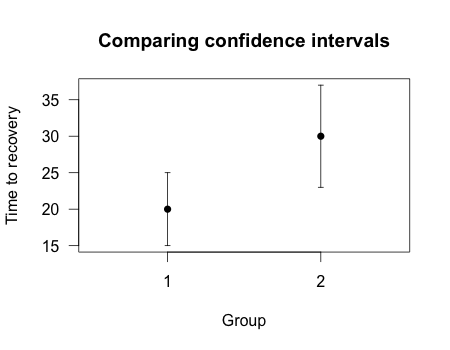
\includegraphics[width=0.5\textwidth]{confidence}
    \caption{Сравнение доверительных интервалов, по оси абсцисс - группы, по оси ординат - время до выздоровления}
    \label{fig5:confidence}
\end{figure}
%%%%%%%%%%%%%%% end of figure %%%%%%%%%%%%%%%%%%%

Представьте, что две нарисованные точки означают примерно оцененное время до выздоравления от некой болезни для двух различных групп пациентов, каждая из которых состоит из десяти пациентов. А эти границы ошибки (линии) могут представлять собой три различные характеристики:

\begin{enumerate}

\item Стандартное отклонение измерений. Подсчитайте разницу между каждым измерением и средним значением, возведите в квадрат эти разницы, а затем подсчитайте среднее значение квадратов и извлеките квадратный корень из получившегося числа. Это и будет стандартное отклонение данной величины и оно измеряет разброс значений по отношению к среднему.

\item Стандартная ошибка какой-либо оценки. Например, возможно, что границы ошибки представляют собой стандартную ошибку среднего. Если бы я решил провести измерения на  множестве различных выборок пациентов, каждая из которых состояла бы из $n$ человек, я могу примерно оценить, что 68\% средних значений времени, требуемого для восстановления, из тех, что я измерил, будут находится в пределах одной стандартной ошибки ``настоящего'' среднего значения времени, необходимого для восстановления. (В случае оценивания средних, стандартная ошибка равна стандартному отклонению, делённому на квадратный корень количества измерений, таким образом, оценка становится тем лучше, чем больше у вас данных, но не слишком быстро.) Многие статистические методы, как, например, регрессия по методу наименьших квадратов, предоставляют оценку стандартной ошибки.   

\item Доверительные интервалы какой-либо оценки. Доверительный интервал уровня 95\%создан математически для того, чтобы включать истинное значение 95 из 100 случайных величин, поэтому в его диапазон входят примерно по два стандартных отклонения в каждом направлении. (Это может быть не совсем верно для более сложных статистических моделей.)  

\end{enumerate}  

Эти три показателя различаются. Стандартное отклонение - это простое измерение моих данных, оно говорит мне о том, как статистическая характеристика, например среднее или наклон наиболее подходящей линии, будет изменяться, если я возьму большое количество пациентов. Доверительный интервал - схожая характеристика, дополнительно гарантирующая, что 95\% доверительных интервалов уровня 95\% должны содержать ``истинное'' значение. 

На графике выше можно увидеть два частично совпадающих доверительных интервала уровня 95\%. Многие ученые, увидев это, сделают вывод об отсутствии статистически значимых различий между группами. В конце концов, группы 1 и 2 \emph{могут и не} различаться - среднее время до восстановления после болезни может быть 25 в обеих группах, нампример, а различия могли проявиться потому что группе 1 в этот раз просто повезло. Но означает ли это, что различие статистически незначимо? Каково будет \emph{\hyperref[chp2:pvalues]{p-значение}}?

В данном случае, $p < 0,05$. Таким образом, существует статистически значимое различие между группами, несмотря на то, что доверительные интервалы частично совпадают.\footnote{Это было подсчитано с использованием t-критерия Стьюдента для независимых выборок, основываясь на стандартной ошибке в 2,5 в группе 1 и 3,5 в группе 2.}

К сожалению, многие ученых пропускают этап тестирования гипотез и просто присматриваются к графикам, чтобы увидеть, пересекаются ли доверительные интервалы. Это даже более консервативный способ - получить результат при котором доверительные интервалы не пересекаются сродни получению $p < 0,01$ в некоторых ситуациях.\cite{schenker_judging_2001} Легко утверждать, что два измерения статистически не различаются в то время, как на самом деле различия есть.  

Противоположно этому, сравнение измерений путем сравнения стандартных ошибок или стандартных отклонений будет также вводить в заблуждение, поскольку границы стандартной ошибки короче границ доверительны интервалов. Два наблюдения могут иметь не пересекающиеся стандартные ошибки, и тем не менее, различия между ними будут статистически не значимыми.

Опрос психологов, нейроученых и медицинских исследователей выявил, что большинство допускают эту простую ошибку помимо того, что многие ученые путают понятия стандартной ошибки, стандартного отклонения и доверительных интервалов.\cite{belia_researchers_2005} Другое исследование научных работ на тему климата обнаружило, что в большинстве статей, сравнивающих 2 группы с использованием границ ошибок, были допущены ошибки.\cite{lanzante_cautionary_2005} Даже вводные учебники по экспериментальной науке, такие как ``Введение в анализ ошибок'', учат студентов принимать решение ``на глаз'', вообще едва упоминая формальную проверку гипотез.   

Конечно, существуют формальные статистические методы, которые создают доверительные интервалы, которые можно сравнивать на глаз, и даже автоматически корректирую множественные сравнения. Например, сравнительные интервалы Гэбриэля легко интерпретировать на глаз.\cite{gabriel_simple_1978}

Частично совпадающие доверительные интервалы не означают, что два значения не различаются статистически. Схожим образом, не пересекающиеся границы стандартных ошибок не означают, что две величины статистически отличаются. Всегда лучше использовать подходящий тест для проверки гипотезы, поверьте, ваш глаз - не самый хороший статистический метод. 
%% Chapter 7 %%%
\chapter{Регрессия к среднему и правила остановки}
\label{chp7}

Медицинские испытания недешевы. Чтобы обеспечить группу пациентов экспериментальными лекарствами и отслеживать проявления их симптомов на протяжении месяцев, может потребоваться значительное количество ресурсов, поэтому многие фармакологические компании разработали т.н. ``правила остановки'', которые позволяют исследователям остановить эксперимент заранее, если очевидно, что экспериментальное лекарство имело значительный эффект. Например, если эксперимент проведён только на половину, но у исследователей уже есть статистически значимые различия в симптомах от действия нового препарата - в таком случае, исследователи могут остановить эксперимент, не стремясь собрать больше данных для подкрепления своих выводов.

Однако, если исследование проведено плохо, это может привести к огромному количеству ложноположительных результатов. 

Например, представьте, что мы сравниваем две группы пациентов, одна их которых принимает лекарство, а другая - плацебо. Мы измеряем уровень какого-нибудь белка в их кровотоке, интерпретируя это как результат действия лекарства. Однако в этом случае, лекарство не вызывает никаких различий: пациенты обеих групп имеют одинаковый средний уровень белка, хотя, естественно, индивидуально уровни слегка различаются. 

Мы начинаем эксперимент с десятью пациентами в каждой группе, и постепенно собираем всё больше данных. В процессе эксперимента, мы проводим $t-$тест для сравнения двух групп и проверки наличия между ними статистически значимых различий в среднем уровне белка. Мы можем увидеть данные, схожие с результатами симуляции на рисунке ниже:


\newpage % делаем разрыв, чтобы картинка была первой на след странице

%%%%%%%%%%%%%% figure 9 %%%%%%%%%%%%%%%%%%5
\begin{figure}[h!]
    \centering
    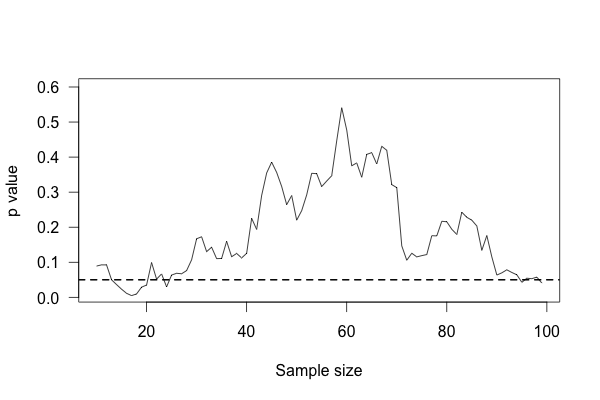
\includegraphics[width=0.8\textwidth]{sample-size}
    %\caption{}
    \label{fig9:sample-size}
\end{figure}
%%%%%%%%%%%%%%% end of figure %%%%%%%%%%%%%%%%%%%

Этот график показывает изменения \emph{p}-значения различий между группами в процессе сбора нами данных, а горизонтальная линия означает уровень значимости $p = 0,05$. На первый взгляд может показаться, что значимых различий нет. Тогда мы собираем больше данных и делаем противоположный вывод. Если бы мы решили остановиться, это было бы заблуждением: мы были бы убеждены в том, что между группами существует значимое различие, в то время как в реальности его нет. Если мы соберём еще больше данных, мы поймем, что были неправы - но в таком случае, есть шанс снова получить ложноположительный результат.  

Можно ожидать, что такое изменение \emph{p}-значения не должно происходить, поскольку реальных различий между группами нет. В конце концов, сбор большего количества данных не должно ухудшать наши выводы, разве нет? И действительно, если мы проведем эксперимент еще раз, мы можем обнаружить, что в начале у групп нет значимых различий, и они не появляются, пока мы собираем данные, или, что сначала у групп есть огромные различия, но в процессе эксперимента они быстро уменьшаются до нуля. Но если мы подождем достаточно долго и будем сравнивать различия после каждого измерения, в конечном итоге мы можем пересечь любую произвольную линию статистической значимости, даже если в реальности различий не будет. Обычно мы не в состоянии собирать данные на бесконечных выборках, поэтому в реальности такого не происходит, но неудачно  составленные и плохо применяемые правила остановки все равно значимо увеличивают количество ложноположительных результатов.\cite{simmons_false-positive_2011}  


Современные клинические испытания часто требуют регистрации используемых статистических протоколов заранее, и, как правило, выбирают только некоторые резальтаты измерения, которые потом тестируют, вместо того, чтобы тестировать после каждого измерения. Это вызывает лишь небольшое увеличение ложноположительных результатов, которое можно корректировать тщательно подобранными уровнями значимости и используя сложные статистические методы.\cite{todd_interim_2001} Но в сферах науки, где протоколы исследования не регистрируются и у исследователей есть возможность выбирать любые методы, которые они считают подходящими, всегда найдется место для таких ошибок.


\section{Преувеличение истины}
\label{chp7:truthinflation}

У медицинских экспериментов также существует тенденция иметь неадекватную статистическую мощность для определения умеренных различий между лекарствами. И они стремятся остановить исследование, как только обнаруживается какой-то результат, но у них не хватает мощности, чтобы обнаружить различия.

Предположим, что лекарство снижает проявление симптомов на 20\% по сравнению с плацебо, но эксперимент, в котором вы пытаетесь это проверить, не имеет адекватной статистической мощности, чтобы определить это различие. Мы знаем, что результаты небольших исследований могут варьировать: удачно собрать в одном эксперименте десять пациентов с более короткой продолжительностью простуды, чем в среднем, легко, но гораздо сложнее собрать десять тысяч таких людей.   

А теперь представьте, что вы проводите множество таких же экспериментов. Иногда вам попадаются не такие удачливые пациенты, и поэтому вы не замечаете никакого статистически значимого улучшения от действия вашего лекарства. Иногда пациенты имеют типично средние показатели, и можно рпонаблюдать снижение симптомов на 20\% благодаря лекарству, но вы игнорируете эти результаты, поскольку у вас недостаточно данных для того, чтобы считать такое улучшение статистически значимым. Иногда пациентам везёт, и их симптомы снижаются более, чем на 20\%, и тогда вы останавливаете эксперимент и говорите:``Смотрите! Лекарство работает!'' 

Вы правильно сделали вывод, что лекарство эффективно, но вы преувеличили размер эффекта. Вы ошибочно поверили в то, что лекарство более эффективно, чем оно есть на самом деле. 

Это часто встречается в фармакологических испытаниях, эпидемиологических исследованиях, исследованиях связей на генном уровне (``ген А является причиной условия В''), психологических исследованиях и в некоторых наиболее цитируемых статьях в медицинской литературе.\cite{ioannidis_why_2008,ioannidis_contradicted_2005} В сферах, где испытания могут проводиться быстро и большим количеством независимых исследователей (как, например, исследования генных связей), самые первые опубликованные результаты зачастую оказываются крайне противоречивыми, поскольку небольшие размеры экспериментов и потребность в статистической значимости приводят к тому, что лишь наиболее выдающиеся результаты в итоге публикуются.\cite{ioannidis_early_2005} 

В качестве бонуса, преувеличение истины можно объединять с правилами предварительной остановки. Если большинство лекарств в клинических испытаниях не настолько эффективны, чтобы оправдать предварительную остановку испытаний, в таком случае большинство экспериментов, остановленных предварительно, будут результатом участия удачливых пациентов, а не действия выдающихся лекарств, - и, останавливая эксперимент, мы фактически лишаем себя возможности собрать дополнительные данные, чтобы это опровергнуть. В обзорах научной литературы сравнивались исследования, остановленные предварительно, с другими, которые изучали те же вопросы, но не были предварительно остановлены, и в большинстве случаев, в предварительно остановленных исследованиях эффект действия тестируемых лекарств был в среднем преувеличен на 29\%.\cite{bassler_stopping_2010} 

Естественно, нам неизвестна ``Истина'' о каждом исследуемом лекарстве, поэтому сложно судить, было ли конкретное исследование предварительно остановлено из-за хорошего лекарства или по желанию исследователей. Во многих исследованиях даже не публикуется изначально планируемый размер выборки или правила остановки, используемые для обоснования прекращения исследования.\cite{montori_randomized_2005} Предварительная остановка исследования не свидетельствует автоматически о том, что его результаты ошибочны, но это определенно наводит на мысль.  



\section{Маленькие крайности}
\label{chp7:littleextremes}

Предположим, что вы ответственны за проведение реформы государственных школ. В рамках изучениях лучших методов обучения, вы обратили внимание на влияние размера школы на результаты тестирования учеников. Лучше ли результаты у маленьких школ, чем у больших? Стоит ли построить большое количество небольших школ или лучше несколько больших?   

Чтобы найти ответы на эти вопросы, вы составляете список лучших школ. В среднем, в школе около 1000 учеников, но практически во всех школах, входящих в десятку лучших по списку, учеников меньше. Похоже, что маленькие школы справляются с обучением лучше, возможно из-за того, что в них формируются условия, при которых учителям удаётся получше узнать учеников и помогать им в индивидуальном порядке.

Затем вы смотрите на худшие из списка школы, ожидая увидеть там большие городские школы с тысячами учеников и перегруженными работой учителями, однако, к вашему удивлению, и там все школы маленькие. 

Что же происходит? Давайте посмотрим на график зависимости результатов тестирования от размера школ:


%\newpage % делаем разрыв, чтобы картинка была первой на след странице

%%%%%%%%%%%%%% figure 10 %%%%%%%%%%%%%%%%%%5
\begin{figure}[h!]
    \centering
    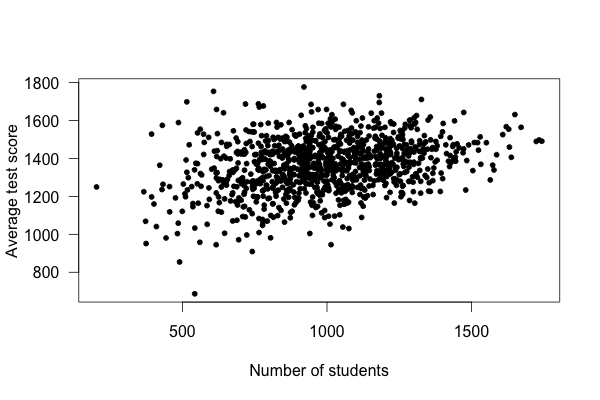
\includegraphics[width=0.8\textwidth]{school-size}
    %\caption{}
    \label{fig9:school-size}
\end{figure}
%%%%%%%%%%%%%%% end of figure %%%%%%%%%%%%%%%%%%%
%%%%%%%%%%%%%%%%%%%%%%%%%%%55
%http://www.statisticsdonewrong.com/_images/school-size.png
%%%%%%%%%%%%%%%%%%%%%%%%%%%%%%%%

У маленьких школ средние значения результатов тестирования значительно варьируются, в основном из-за того, что у них меньше учеников. Меньшее количество учеников означает меньшее наличие данных для того, чтобы установить ``истинные'' результаты работы учителей, и поэтому средние значения результатов сильно разнятся. Чем крупнее школа, тем меньше варьируют результаты, а среднее значение, в действительности, даже увеличивается.  

В этом примере использовались данные симуляции, но он основан на настоящих (и неожиданных) результатах наблюдения за государственными школами Пенсильвании.\cite{wainer_most_2007}

Другой пример: В Соединенных Штатах, наименьший уровень заболевания раком почки, как правило, имеют сельские округа Среднего Запада, а также южные и западные штаты. Почему так? Можно найти несколько объяснений, например: деревенские жители больше заняты физическим трудом, дышат менее загрязненным воздухом и, возможно, ведут менее напряженный образ жизни. Вероятно, эти факторы снижают показатели встречаемости рака. 

С другой стороны, округа с самыми высоким уровнем заболевания раком почки выступают те же сельские округа Среднего Запада, южные и западные штаты.

Проблема, естественно, заключает в том, что в сельской местности живёт меньше людей. Единственный пациент с диагнозом рака почки в округе, где живет всего 10 человек, даст этому округу самый высокий уровень заболевания раком почки по всей стране. Следовательно, маленькие округа имеют значительно более варьируемые показатели заболевания раком почки, просто потому, что у них так мало жителей.\cite{gelman_all_1999}


%% Chapter 8 %%%
\chapter{Свобода исследователя: хорошие сомнения? }
\label{chp8}

Существует распространенное заблуждение о том, что статистика скучна и однообразна. Соберите как можно больше данных, загрузите цифры в $Excel$, $SPSS$ или $R$, и пинайте программу до тех пор, пока она не выдаст какие-нибудь красочные графики или диаграммы. Готово! Все, что остается статистикам, - это считывать результаты.

Однако, придётся выбирать, какие методы и команды использовать. Два исследователя, ищущих ответы на один и тот же вопрос, могут использовать совершенно разные методы статистического анализа. Нужно принимать множество решений:


\begin{enumerate}
	\item Какие переменные мне нужно учитывать? В медицинских испытаниях, например, стоит контролировать возраст пациентов, пол, вест, ИМТ, предыдущую медицинскую историю, курение, использование наркотиков или результаты медицинских тестов, проведённых до начала исследования. Какие из этих факторов важны, а какие можно игнорировать?

	\item Какие случаи можно исключить? Если я тестирую планы питания, возможно, я хочу исключить испытуемых, у которых в процессе исследования появилась неконтроллируемая диарея, так как их результаты будут выходить за рамки нормы.

	\item Что делать с выбросами? По неизвестным причинам, среди результатов всегда будут некоторые выпадающие из нормы, и, возможно, мне придется их исключить или анализировать отдельно. Какие случаи тогда можно считать выбросами и что мне с ними делать?

	\item Как мне определить группы? Например, я, возможно, хочу разделить испытуемых на группы ``нормальных'', ``с избыточным весом'' и ``с недостаточным весом''. Как определить границы групп? Что мне делать с мускулистыми бодибилдером, чей ИМТ находится в диапазоне значений группы ``с избыточным весом''?

	\item Что насчёт отсутствующих данных? Допустим, я пытаюсь оценить уменьшение распространения рака путем тестирования нового лекарства. Я провожу испытания в течении пяти лет, но у некоторых пациентов опухоли возвращаются через шесть или восемь лет, а в мои данные этого не будут содержать. Как мне это учитывать при оценке эффективности лекарства? 

	\item Сколько данных я должен собрать? Стоит ли мне остановиться, как только я получу определённый результат, или следует продолжать до тех пор, пока я не соберу все данные, как было запланировано?

	\item Как мне оценить полученные результаты? Действие лекарства можно оценить с помощью индивидуальных опросов пациентов, результатов испытаний, преобладания определенного симптома или, например, продолжительностью болезни.

\end{enumerate}

Прежде, чем появятся результаты, можно потратить много времени на определение того, какие методы будут наиболее уместны в данной ситуации. Научные статьи обычно содержат объяснение того, какие методы статистической обработки были использованы, но они практически никогда не объясняют причину выбора именно этого метода по сравнению с другими или какие результаты могли получить исследователи, используя другие методы. Исследователи вольны выбирать методы, которые они считают подходящими, - и, хотя они могли сделать правильный выбор, что было бы, анализируй они эти данные по-другому?    

При моделировании можно получить различающиеся в два раза размеры эффекта просто путем регулирования различных переменных, исключения определенных наборов случаев из анализа и обработки выбросов другим способом.\cite{ioannidis_why_2008} Размер эффекта - это та самая важная цифра, которая показывает, сколько различий привносит ваше лекарство. Таким образом, очевидно, что свобода выбирать, как анализировать свои данные, даёт вам немалый контроль над получаемыми результатами!  

Наиболее важное следствие такой статистической свободы заключается в том, что исследователи могут выбирать любимые методы анализа, произвольно получая статистически значимые результаты, манипулируя и играя с данными до тех пор, пока что-нибудь не появится. Моделирование показывает, что оценки ложно положительных результатов могут вырасти до 50\% для конкретного набора данных просто позволяя исследователям использовать разные статистические методы до тех пор, пока какой-нибудь не сработает.\cite{simmons_false-positive_2011}

Медицинские исследователи разработали способ предотвращения такой ситуации. От исследователей обычно требуют составить план протокола клинических испытаний, в котором бы объяснялось каким образом данные будут собираться и анализироваться. Поскольку протокол составляется до того, как исследователи увидят какие либо данные, они в принципе не могут сделать анализ наиболее благоприятным для себя. К сожалению, многие исследования отступают от протоколов и проводят различные анализы данных, делая возможным появление феномена ошибки экспериментатора.\cite{chan_discrepancies_2008,chan_empirical_2004} Во многих других исследовательских сферах в принципе отсутствует требование публикации протоколов исследования.

Распростанение статистических методов дало нам множество полезных инструментов, но, похоже, их используют в качестве тупых предметов. Надо просто бить данные до тех пор, пока они не признаются.

%% Chapter 9 %%%
\chapter{Ошибки делают все}
\label{chp9}

До сих пор, я предполагал, что ученые способны выполнять статистические вычисления с идеальной точностью и ошибаться могут только в выборе подходящих для этих вычислений цифр. Ученые могут неправильно использовать результаты статистического анализа или не в состоянии выполнить соответствующие расчеты, но они ведь могут, как минимум, правильно рассчитать \emph{p-}значение?

Возможно, нет. 

Обзоры статистически значимых результатов, представленных в медицинских и психологических исследованиях, показывают, что многие \emph{p-}значения ошибочны, и некоторые статистически незначимые результаты на самом деле значимы, если правильно их пересчитать.\cite{gotzsche_believability_2006,bakker_misreporting_2011} Другие обзоры находят примеры неверной классификации данных, ошибочного дублирования данных, использование полностью неверных наборов данных в анализ и других ошибок, - все спрятаны в статьях, которые не содержат описания проведённого анализа, достаточно подробного для того, чтобы эти ошибки можно было легко заметить.\cite{baggerly_deriving_2009,gotzsche_methodology_1989} 

Солнечный свет - лучшее средство дезинфекции, и многие ученые призывали к тому, что экспериментальные данные должны быть доступны в интернете. В некоторых областях, это стало распространенной практикой: существуют базы данных генных последовательностей, белковых структур, астрономических наблюдений и коллекции данных земных наблюдений, содержащие вклад тысяч различных ученых. Многие другие сферы науки, однако, не могут поделиться своими данными ввиду непрактичности (данные физики элементарных частиц могут содержать терабайты информации), невозможности разглашения (медицинские исследования), отсутствия финансирования или технической поддержки или просто исходя из желания сохранить контроль над данными и всеми открытиями, появляющиеся в результате их анализа. И даже если бы все данные были доступны, стал бы кто-нибудь их анализировать с целью поиска ошибок?   

Схожим образом, ученые в некоторых областях стали делать свой статистический анализ общедоступным путём использования умных технологических инструментов. Например, инструмент под названием Sweave позволяет легко встраивать статистический анализ, сделанный с исопльзованием популярного языка программирования $R$, в научные статьи, написанные с помощью \LaTeX, считающийся стандартом для написания научных и математических публикаций. Результат выглядит точно также, как и любая научная статья, но другой ученый, прочитавший публикацию и заинтересовавшийся используемыми методами, может скачать исходный код, в котором показано, каким образом были проведены все расчеты. Но будут ли ученые пользоваться такой возможностью? Никто же не достигает научной славы, проверяя код на наличие опечаток.

Другим решением может выступать повторение исследования. Если ученые тщательно воссоздадут ход эксперимента других ученых и подтвердят их результаты, будет намного проще исключить возможность опечатки, которая может привести к ошибочным результатам. Повторение также устраняет случайные ложно положительные результаты. Многие ученые утверждают, что экспериментальное повторение - это основа науки, поскольку ни одна новая идея не принимается до тех пор, пока она не была независимо проверена и перепроверена учеными по всему миру и оказалась способной выдерживать критику.  

Это не совсем верно: ученые часто принимают результаты предыдущих исследований на веру, хотя иногда решают методично перепроверять предыдущие работы. Например, один новый проект ставит своей целью воспроизвести результаты исследований из крупных психологических журналов, чтобы определить, какое количество статей выдерживают проверку временем и по каким характеристикам можно предсказать, насколько статья способна выдержать последующие перепроверки.\footnote{\href{http://openscienceframework.org/reproducibility/}{The Reproducibility Project}} 

В другом примере, исследователи рака из компании Amgen провели повторно 53 выдающихся доклинических исследования рака. (``Доклинические'' исследования в данном случае подразумеваются исследования, в которых не участвовали пациенты, поскольку в них проверялись новые и неподтвержденные идеи.) Несмотря на сотрудничество с авторами оригинальных статей, исследователям из Amgen удалось повоторить только шесть исследований.\cite{begley_drug_2012} Исследователи из компании Bayer сообщали о таких же проблемах в процессе тестирования возможных новых лекарств, обнаруженных в опубликованных статьях.\cite{prinz_believe_2011}

Это тревожит. Прослеживается ли эта тенденция во всех видах медицинских исследований? По-видимому, да: из списка наиболее цитируемых статей по медицине, четверть оказались непроверенными после публикации, а треть работ содержали преувеличенные или ошибочные результаты, как показали последующие исследования.\cite{ioannidis_contradicted_2005} Это не настолько экстремальные результаты, как у исследователей из Amgen, но заставляет задуматься, какие еще серьёзные ошибки остаются незамеченными в важных иследованиях. Повторение исследования - всё еще не самая распространенная практика, как, возможно, нам бы хотелось, и результаты ее не всегда приятны.


%% Chapter 10 %%%
\chapter{Скрываем данные}
\label{chp10}

\begin{chapquote}{Эрик С. Рэймонд}
``При достаточном количестве глаз, все ошибки выплывают на поверхность.''
\end{chapquote}


Ранее мы говорили о наиболее распространенных ошибках, которые допускают учёные, и о том, что наилучший способ их обнаружить - тщательное изучение извне. Экспертная оценка, в некоторой степени этому способствует, однако у человека, проводящего оценку, недостаточно времени для того, чтобы подробно проанализировать все данные повторно и проверить все исходные коды анализа на ошибки, - рецензенты могут лишь проверить правильность выбранной методологии исследования. Иногда они замечают очевидные ошибки, но едва заметные проблемы, как правило, пропускают. \cite{schroter_what_2008}  


Поэтому многие рецензируемые журналы и профессиональные сообщества требуют от исследователей предоставлять другим исследователям доступ к своим данным по запросу. Полные наборы данных, как правило, слишком большие по размеру, чтобы их можно было напечатать на страницах журнала, поэтому авторы лишь публикуют свои результаты в статьях, а копию данных отправляют другим исследователям по запросу. Возможно, другие исследователи смогут обнаружить ошибку или незамеченную закономерность.

Теоретически, именно так это и должно происходить. В 2005 году Джелте Уичертс с коллегами из университета Амстердама решили проанализировать недавно опубликованные статьи в нескольких знаменитых журналов Американской Психологической Ассоциации, чтобы узнать об использованных в них статистических методах. Они выбрали журналы АПА отчести потому, что это сообщество требует от авторов статей согласие на предоставление собранных в рамках исследования данных другим психологам, стремящихся проверить их результаты. 

Шесть месяцев спустя они смогли получить данные только по 64 исследованиям из 249 анализируемых. Почти три четверти авторов статей так и не прислали им свои данные. \cite{wicherts_poor_2006} 

Конечно, учёные - занятые люди и, возможно, у них просто не нашлось свободного времени, чтобы собрать свои даные, подготовить пояснительные документы, описывающие значения каждой переменной и каким образом она была измерена, и так далее.

Уитчерс и коллеги решили это проверить. Они тщательно просмотрели все исследования на наличие наиболее распространенных ошибок, которые можно было бы заметить в процессе чтения статьи, таких как: противоречивые статистические результаты, неправильное применение различных статистических тестов и обычных опечаток. По крайней мере, в половине статей содержались ошибки, как правило, незначительные, однако 15\% статей содержали описание не менее одного статистически значимого результата, который был значимым исключительно из-за ошибки. 

Далее, они искали корреляцию между этими ошибками и нежеланием авторов делиться своими данными, и, как оказалось, между ними существовала четкая связь. Авторы, отказавшиеся делиться своими данными, были в большей степени склонны допускать ошибку в своей статье, и статистические обоснования их выводов были, как правило, слабее. \cite{wicherts_willingness_2011} Поскольку большинство авторов отказались предоставлять свои данные, Уитчерс не мог провести более детальный поиск статистических ошибок, которых могло оказаться гораздо больше.

Это, конечно, не доказательство того, что авторы скрывали свои данные, боясь обнаружения их ошибок, или что они вообще знали о наличии этих ошибок. Наличие корреляции не подразумевает наличие причинно-следственной связи, но в данном случае корреляция явно намекает ``внимательно посмотри сюда.''\footnote{Шутка бесстыдно украдена из альтернативного варианта комикса \href{http://xkcd.com/552/}{http://xkcd.com/552/}}



\section{Просто опустите подробности}
\label{chp10:leaveoutdetails}

Придирчивые статистики тянут вас на дно, указывая на недостатки вашей статьи? Существует одно простое решение: публикуйте как можно меньше подробностей! Они не смогут найти ошибки, если вы не скажете как вы оценивали свои данные.

Я не утверждаю всерьёз, что злые ученые делают это намерянно, хотя, возможно, некоторые делают. Чаще детали опущены просто потому, что авторы забыли включить их в статью или в виду того, что ограничения журнала на размер статьи заставили так поступить.

Исследование можно оценить, чтобы понять, что было исключено. Учёные, ведущие медицинские испытания, должны предоставлять подробные планы исследования экспертным советам по этике до начала испытаний, поэтому одна группа исследователей получила коллекцию таких планов от одного  экспертного совета. В этих планах указывалось, какие результаты исследования будут измеряны: например, можно отслеживать различные симптомы, чтобы пронаблюдать, оказывало ли на них влияние тестируемое лекарство. Затем исследователи разыскали опубликованные результаты этих планируемых исследований и посмотрели, насколько хорошо эти результаты были представлены.   

Примерно половина планируемых результатов никогда так и не появились в научных статьях рецензируемых журналов. Многие из них оказались статистически незначимыми, поэтому были просто скрыты. Другая большая часть результатов была опубликована без подробностей, что исключало возможность в дальнейшем использовать эти результаты для мета-анализа. \cite{chan_empirical_2004} 

%убрал сноску №2, не вижу смысла ее переводить %%%

Другие обзоры сталкивались с похожими проблемами. Обзор клинических испытаний обнаружил, что большинство исследований опускают важные методологические детали, как например, \hyperref[chp7]{правила остановки} или \hyperref[chp3]{расчеты мощности}, - это свойственно, в большей степени, небольшим специализированным журналам, нежели большим общемедицинским журналам. \cite{huwiler-muntener_quality_2002}

Журналы по медицине пытаются бороться с этой проблемой путем стандартизации отчетов о результатах, таких как список \href{http://www.consort-statement.org/}{CONSORT}. Авторы должны следовать требованиям списка до момента предоставления работы на рассмотрение, а редакторы проверяют, включены ли в статью все необходимые детали. Этот список, похоже, работает: исследования, опубликованные в журналах, которые следуют рекомендациям от CONSORT, как правило, предоставляют больше существенных подробностей об исследовании, хотя и не все. \cite{plint_does_2006} К сожалению, стандарты не всегда последовательно применяются и некоторым работам удается проскочить мимо них с отсутствующими в исследовании деталями. \cite{mills_analysis_2005} Редакторам журналов придётся приложить больше усилий для соблюдения стандартов отчётности.

По-видимому, с опубликованными статьями дела обстоят не очень хорошо. А с неопубликованными исследованиями?


\section{Наука в картотеке}
\label{chp10:sciencecabinet}

Ранее мы видели влияние \hyperref[chp5:try-again]{множественных сравнений} и \hyperref[chp7:truthinflation]{преувеличения истины} на результаты исследования. Эти проблемы возникают, когда в исследованиях проводятся многочисленные сравнения с низкой статистической мощностью, повышая, тем самым, количество ложноположительных результатов и оценки размеров эффекта, и такие исследования встречаются в публикациях постоянно.

Однако, не каждое исследование публикуется. Мы всегда видим только часть медицинских исследований, например, потому что немногие учёные публикуют результаты из разряда ``Мы протестировали данное лекарство и непохоже, что оно сработало.''

Рассмотрим пример: изучение опухолевого супрессора белка TP53 и его влияния на рак головы и шеи. Ряд исследований предполагали, что измерение TP53 может быть использовано для прогнозирования показателей смертности от рака, поскольку он участвует в регуляции роста и развития клеток, и, следовательно, должен функционировать правильно, для предотвращения рака. Когда все 18 опубликованных исследований по изучению TP53 и рака были проанализированы вместе, в результате была получена статистически значимая корреляция: измеряя TP53 можно явно определить, насколько вероятно умереть от опухоли.

Но, предположим, что мы откопали \emph{неопубликованные} результаты исследований TP53: данные, которые упоминались в других исследованиях, но не были опубликованы и проанализированы. Добавьте эти данные к уже имеющимся, и статистически значимый эффект исчезает. \cite{kyzas_selective_2005} В конце концов, немногие авторы потрудились опубликовать данные, показывающие отсутствие корреляции, поэтому в мета-анализе использовалась фактически смещенная выборка. 

Аналогичное исследование рассматривало ребоксетин - антидепрессант, продаваемый компанией Pfizer. Несколько опубликованных исследований предполагали его эффективность по сравнению с плацебо, что привело к тому, что в нескольких европейских странах оно было одобрено для лечения пациентов в состоянии депрессии. Немецкому институту Качества и Эффективности в Здравоохранении, ответственному за оценку медицинских лекарств, удалось получить неопубликованные данные клинических испытаний от Pfizer - в три раза больше данных, чем когда-либо опубликованных - и тщательно их проанализировать. В результате, ребоксетин оказался неэффективным. Pfizer просто убедил общественность в том, что антидепрессант эффективен, пренебрегая упоминанием исследований, которые доказывали обратное. \cite{eyding_reboxetine_2010}

Эта проблема широко известна под названием ``ошибка публикации'' или ``проблема картотечного ящика'': многие исследования остаются неопубликованными, ``хранятся в ящиках'' в течении многих лет, несмотря на ценные данные, которые в них содержатся.

Проблема заключается не просто в смещении на опубликованные результаты. Неопубликованные исследования ведут к дублированию усилий - если другие учёные не знают, что вы провели исследование, они вполне могут снова его провести, тратя напрасно деньги и усилия. 

Регуляторы и научные журналы пытались решить эту проблему. Управление по санитарному надзору за качеством пищевых продуктов и медикаментов США (FDA) требует, чтобы определённые виды клинических испытаний были зарегистрированы на их веб-сайте \href{https://clinicaltrials.gov/}{ClinicalTrials.gov} до начала испытаний, а также, чтобы результаты этих испытаний были опубликованы в течении года после окончания испытаний. Точно также, Международная комиссия редакторов медицинских журналов в 2005 году объявила, что они не будут публиковать исследования, которые не были предварительно зарегистрированы.

К сожалению, обзор 738 зарегистрированных клинических испытаний обнаружил, что только 22\% соответствовали законным требованиям к публикации. \cite{prayle_compliance_2012} Управление по санитарному надзору (FDA) не оштрафовала ни одну фармацевтическую компанию за несоблюдение их требований, а журналы всё еще не требуют предварительной регистрации испытаний. И большинство исследований просто исчезают.

%% Chapter 11 %%%
\chapter{К чему мы пришли?}
\label{chp11}

Я обрисовал мрачную картину. Любой может увидеть мелкие детали в публикациях и составить из них огромный список ошибок. Имеют ли они какое-нибудь значение?

Да, имеют. Иначе я бы не написал всё это.

Знаменитая статья Джона Иоаннидиса ``Почему большинство опубликованных результатов исследований являются ложью''\cite{ioannidis_why_2005} была обоснована и затрагивала в большей степени математические расчеты, нежели эмпирические проверки исследовательских результатов. Если большинство научных статей имеют низкую статистическую мощность - \hyperref[chp3]{а они имеют}, в то время, как у исследователей остается свобода выбора из множества различных методов анализа для получения благоприятных результатов, \hyperref[chp8]{что они и делают}; когда большинство тестируемых гипотез ложны и большинство истинных гипотез соответствуют очень слабым по силе эффектам, мы математически детерминированы на получение массы ложно положительных результатов. 

Но если вам нужен эмпиризм - можете его получить, как сказали Джон Иоаннидис и Джонатан Шоэнфельд. Они изучали вопрос ``Связано ли всё, что мы едим, с раком''\cite{schoenfeld_is_2013}\footnote{Это важная часть текущего онкологического проекта \href{http://dailymailoncology.tumblr.com/}{Oncological Ontology} по классификации всего на две категории: то, что лечит рак, и то, что его является его причиной.} Выбрав пятьдесят популярных ингридиентов из кулинарной книги, они занялись поиском исследований, связывающих их с показателями заболевания раком, - и обнаружили 216 исследований, описывающих сорок различных ингредиентов. Естественно, большинство исследований противоречили друг другу. Среди исследований оказалось как много защитников, так и противников большинства ингредиентов: одни утверждали, что ингредиент повышает риск заболевания раком, другие постулировали обратное. Большая часть статистических данных было очень слабым, а мета-анализы, как правило, показывали гораздо меньший размер эффекта, в отличие от результатов оригинальных исследований.


Конечно, тот факт, что данные последующих исследований и мета-анализов противоречат результатам одной статьи, не предотвращает дальнейшее её цитирование в других статьях, считающих её результаты истинными. Даже эффекты, которые вступают в противоречие с последующими многочисленными испытаниями с недвусмысленными результатами, всё равно часто цитируются пять или десять лет спустя учёными, которые, по-видимому, не замечают, что эти результаты являются уже ложными.\cite{tatsioni_persistence_2007} Конечно, новые находки получают широкую огласку в прессе, в то время как противоречия или исправления едва ли вообще упоминаются.\cite{gonon_why_2012} Сложно винить учёных за то, что они не в курсе.

Не стоит забывать и о просто ошибочных результатах. Плохие стандарты отчетности в медицинских журналах означают, что исследователи, тестирующие новое лекарство от шизофрении, могут пренебречь включением в статью шкалы, по которой они оценивали проявление симптомов, - неиссякаемый источник ошибки, поскольку результаты с неопубликованными шкалами, как правило, выглядят лучше тех, для получения которых использовались проверенные тесты.\cite{marshall_unpublished_2000} Другие медицинские исследования просто \hyperref[chp10:leaveoutdetails]{не упоминают определённые результаты}, если они не интересны или не благоприятны исследованию, продуцируя, таким образом, ошибки в последующих мета-анализах. По оценкам, примерно треть мета-анализов страдают от этой проблемы.\cite{kirkham_impact_2010}

В другом обзоре сравнивались мета-анализы с последующими крупными рандомизированными контроллируемыми испытаниями, которые считаются золотым стандартом в медицине. В более чем трети случаев, результат рандомизированного испытания плохо соответствовал мета-анализу.\cite{lelorier_discrepancies_1997} В другиъ сравненияъ мета-анализов с последующими исследованиями было обнаружено, что большинство результатов были преувеличены, примерно пятая часть которых представляла ложно положительные.\cite{pereira_statistically_2011}

Также, не стоит забывать о множестве научных трудов по физике, которые злоупотребляют доверительными интервалами.\cite{lanzante_cautionary_2005} Или о рецензируемой статье по психологии, в которой якобы представлены доказательства в пользу психических сил, основанные на неконтроллируемых множественных сравнениях в поисковых исследованиях.\cite{wagenmakers_why_2011} Неудивительно, что результаты не поддаются повторению - учеными, которые, кажется, не рассчитали статистическую мощность своих тестов.\cite{galak_correcting_2012}

У нас есть проблема. Давайте работать над её решением.

%% Chapter 12 %%%
\chapter{Что можно сделать?}
\label{chp12}

На протяжении этой книги мы обсуждали большое количество статистических проблем, которые возникают во многих областях науки: медицине, физике, климатических исследованиях, нейронауках, и многих других. Любой исследователь, использующий статистические методы для анализа данных, может допустить ошибку, и, как мы уже видели, многие допускают. Что мы можем с этим сделать?


\section{Статистическое обучение}
\label{chp12:statisticaleducation}

Большинство американских студентов имеют лишь минимальное статистическое образование - один или два обязательных курса, а у многих вообще ни одного. И даже если студенты прошли обучение по курсу, преподаватели отмечают, что они не способны применять статистические понятия к научным вопросам, поскольку никогда не понимали или просто быстро забывали соответствующие методы. Это необходимо изменить. Практически каждая научная дисциплина зависит от статистического анализа экспериментальных данных, а статистические ошибки просто обесценивают время исследователей и финансовые гранты. 

В некоторых университетах экспериментировали, пытаясь совмещать статистические курсы и научные занятия, чтобы студенты могли сразу применять свои статистические знания к проблемам в изучаемых научных сферах. Предварительные результаты показывают, что это работает: студенты узнают и запоминают больше статистических методов, и меньше жалуются на то, что их принуждают изучать статистику.\cite{metz_teaching_2008} Другие университеты должны перенять такие методы, используя концептуальные тесты, чтобы определить, какие методы работают лучше всего.  

Учебные материалы должны быть также более доступными. Я познакомился со статистикой, когда мне нужно было проанализировать данные, полученные в лаборатории, и я не знал как это сделать; пока статистическое обучение не станет повсеместным, многие студенты будут оказываться в схожих ситуациях - и им нужны будут источники информации. Такие проекты, как \href{https://www.openintro.org/stat/textbook.php}{OpenIntro Stats}, выглядят многообещающими, и, я надеюсь, в ближайшем будущем их станет еще больше.


\section{Научные публикации}
\label{chp12:sciencepublishing}

Научные журналы медленно добиваются прогресса в решении тех проблем, которые я обсуждал. Такие принципы, как CONSORT для рандомизированных испытаний, делают ясным, какая информация требуется должна быть в публикуемой статье, чтобы она была воспроизводимой. К сожалению, как мы уже видели ранее, эти принципы предписываются нечасто. Мы должны продолжать оказывать давление на журналы, чтобы они требовали от своих авторов соблюдения строгих стандартов.

Главные журналы должны возглавить эту тенденцию. Журнал \emph{Nature} уже так сделал, объявив новый \href{http://www.nature.com/authors/policies/checklist.pdf}{перечень требований}, которому авторы должны полностью следовать, чтобы их статьи были опубликованы. В этот перечень будут входить требования публикации размеров выборки, подсчета статистической мощности, регистрационные номера клинических испытаний, полный список требований CONSORT, корректировка для множественных сравнений и обмен данными и исходным кодом. Этот перечень покрывает практически все проблемы, рассмотренные в этой книге, за исключением \hyperref[chp7]{правил остановки} и обсуждения причин отклонения от зарегистрированного \hyperref[chp8]{протокола} исследования. \emph{Nature} также сделает доступными статистические консультации для статей, если потребуется. 

Если эти принципы сделать законом, тогда в результате мы получим более надежные и воспроизводимые научные исследования. Другие журналы должны делать тоже самое.


\section{Ваша задача}
\label{chp12:yourjob}

Ваша задача может быть выражена в виде четырёх простых шагов:

\begin{enumerate}

	\item Прочитайте хорошую книгу по статистике или пройдите хороший курс. Практикуйтесь.
	\item Планируйтесвой анализ данных тщательно и аккуратно, стараясь избегать заблуждений и ошибок, о которых вы узнали.
	\item Если вы обнаружили знакомую ошибку в научной литературе, такую как, например, неправильную интерпретацию \emph{p-}значений, - просто ударьте виновного по голове своим учебником по статистике. Это поможет. % или "В терапевтических целях".
	\item Добивайтесь изменений в научном образовании и публикациях. Это наше исследование. Давайте не облажаемся.

\end{enumerate}


%% Chapter 13: Conclusion %%%
\chapter*{Заключение}
\label{chp13}
\addcontentsline{toc}{chapter}{Заключение}

Остерегайтесь ложной уверенности. У вас может довольно быстро появиться самодовольное чувство удовлетворения от того, что ваша работа всегда идеальна, в отличие от других. Но в этой книге не было полного введения в математику, стоящую за анализом данных. Есть много других способов испортить статистику и за пределами этих простых концептуальных ошибок.

Ошибки будут происходить часто, поскольку лишь некоторые научные бакалаврские программы или медицинские школы требуют изучения курсов по статистике и дизайну экспериментов, - и некоторые вводные курсы по статистике опускают рассмотрение вопросов статистической мощности и множественных следствий. Это выглядит достаточным, несмотря на первостепенную роль данных и статистического анализа в стремлениях и поисках современной науки; мы ведь не принимаем докторов, у которых нет опыта работы с рецептурными лекарствами, так почему мы принимаем ученых, не имеющих статистической подготовки? Ученым нужно формальное статистическое обучение и консультации. Цитата:\\

%\newline

\begin{chapquote}{Р.А. Фишер, популяризатор \emph{p}-значения}
``Проконсультироваться с статистиком после того, как эксперимент был закончен, - это как попросить его провести посмертное вскрытие. Он, возможно, скажет, из-за чего умер эксперимент.''
\end{chapquote} 

Журналы могут отказывать в публикации исследованиям с статистическим анализом низкого качества, а новые требования и протоколы могут устранить некоторые проблемы, но никакого улучшения в планировании экспериментов и анализе данных не будет до тох пор, пока у нас не будет ученых, обученных в соответствии с принципами статистики. Лишь продолжатся всепоглощающие поиски статистической значимости.

Изменения не будут простыми. Строгие статистические стандарты не даются даром: например, если ученые начнут регулярно делать подсчеты статистической мощности, скоро обнаружится, что им нужны значительно б\emph{о}льшие размеры выборок, чтобы достичь убедительных выводов. Клинические испытания не бесплатны, и более дорогая стоимость исследований означает меньшее количество опубликованных испытаний. Вы можете возразить, что научный прогресс будет излишне замедлен - но разве не хуже строить наш прогресс на фундаменте необоснованных результатов?

Для студентов, изучающих науку: вкладывайте в статистические курсы, пока у вас есть возможность. Исследователям: вкладывайте в обучение, хорошую книгу и полезный статистический совет. И когда в следующий раз вы услышите, как кто-то говорит: ``Результат оказался значимым на уровне $p<0,05$, т.е. есть лишь 1 шанс из 20, что это случайность!'', - пожалуйста, стукните его по голове учебником по статистике за меня.

\textbf{Отказ от ответственности}: Советы, приведённые в этом руководстве, не могут заменить консультации квалифицированного специалиста по статистике. Если вам кажется, что вы страдаете от любой серьезной статистической ошибки, пожалуйста, немедленно проконсультируйтесь со статистиком. Я не несу никакой ответственности в случае, если в результате использования данного веб-сайта и руководства пострадало ваше достоинство.

Использование этого руководства в целях оправдания отрицания результатов научного исследования без подробного рассмотрения любых доказательств будет основанием получить сверху по голове очень большим учебником по статистике. Это руководство должно помочь вам находить статистические ошибки, а не позволить вам выборочно игнорировать те части науки, которые вам не нравятся.


%%% Конец основного текста %%%%


%%%%%%%%%%%%%%%%%%%%%%%%%%%%%%
%%% Начало библиографии %%%%%
\cleardoublepage
\phantomsection
\addcontentsline{toc}{chapter}{Список литературы}
\bibliography{biblio/SDW}{}
\bibliographystyle{abbrv}
%\fontencoding{T1}\selectfont 




%\printindex % печать предметного указателя здесь
%\appendix
%\backmatter
\end{document}